\documentclass[a4paper]{article}

\usepackage{lmodern}

%% Language and font encodings
\usepackage[french]{babel}
\usepackage[utf8x]{inputenc}
\usepackage[T1]{fontenc}

%% Sets page size and margins
\usepackage[a4paper,top=3cm,bottom=3cm,left=2cm,right=2cm,marginparwidth=2cm]{geometry}

%% Useful packages
\usepackage{amsmath}
\usepackage{graphicx}
\usepackage[colorinlistoftodos]{todonotes}
\usepackage[colorlinks=true, allcolors=black]{hyperref}
\usepackage{fourier-orns}
\usepackage{titlesec}
\usepackage{fancyhdr}
\usepackage{fancyvrb}
\usepackage{enumitem}
\usepackage{float}
\usepackage{libertine}
\pagestyle{fancy} 
\setcounter{tocdepth}{5}

%% Tikz stuff
\usepackage{tikz}
\usetikzlibrary{calc, arrows}
\tikzstyle{incolore} = [rectangle, rounded corners, draw=black, minimum height=1cm, minimum width=3cm, text width=3cm, text centered]

\newcommand{\hsp}{\hspace{20pt}}
\newcommand{\HRule}{\rule{\linewidth}{0.5mm}}

% Défini la règle d'en-tête
\renewcommand{\headrulewidth}{1pt}
\fancyhead[C]{} 
\fancyhead[L]{}
\fancyhead[R]{\footnotesize{\leftmark}}

% Défini la règle de fond de page
\renewcommand{\footrulewidth}{1pt}
\fancyfoot[C]{} 
\fancyhead[L]{}
\fancyfoot[R]{\thepage}

\definecolor{Zgris}{rgb}{0.87,0.85,0.85}

\usepackage{eso-pic,graphicx}
\usepackage{xcolor}
\newcommand{\bgimg}[1]{
    \AddToShipoutPicture
    {
        \put(\LenToUnit{0 cm},\LenToUnit{0 cm})
        {
            \includegraphics[width=\paperwidth,height=\paperheight]{#1}
        }
    }
}

\begin{document}
\begin{titlepage}
    \begin{sffamily}
        \begin{center}
            \textnormal{}\\[6.5cm]
            \HRule \\[0.4cm]
            { \Huge \bfseries Synthèse\\ Télécommunication\\ [0.4cm] }
            \HRule \\[3cm]
            \Large
            Premier Bloc\\
            Sécurité des systèmes\\
            Année académique 2019-2020\\[0.5cm]
            \emph{Rédigé par}\\
            \emph{Roumache Grégoire et Sénéchal Julien}
            \vfill
            {\large 22 Mai 2020}
        \end{center}
    \end{sffamily}
\end{titlepage}

\section{Les ondes électromagnétiques}
\begin{center} \textit{Champ magnétique + Champ électrique = Onde électromagnétique} \end{center}
Les 2 types de champs perturbent mutuellement le champ de l'autre. Ce qui crée le champ électromagnétique !
Contrairement à une onde mécanique, celle-ci peut se déplacer dans le \textbf{vide}. 
Dans le vide, la vitesse de cette onde est égale a la vitesse de la lumière ($3\times10^{8} \; \frac{m}{s}$).\\[0.2cm]
\begin{itemize}
  \item Un champ est une partie de l'espace dont chaque point possède une propriété que l'on étudie.
  \item Les 2 champs (électrique et magnétique) sont perpendiculaire l'un à l'autre.
  \item Le champ électrique et le champ magnétique sont deux phénomènes distincts :
  \begin{itemize}
    \item Le champ électrique varie selon la tension électrique
    \item Le champ magnétique varie selon l'intensité du courant électrique\\[0.2cm]
  \end{itemize}
  
\end{itemize}
\par
Caractéristiques de l'onde :
\begin{itemize}
  \item Sa vitesse de propagation ($c$) : $3\times10^{8}\frac{m}{s}$ dans le vide
  \item Sa fréquence ($f$) : Le nombre de maxima de champ par seconde en un point donné (en \emph{Hz})
  \item La longueur d'onde ($\lambda$) : Distance entre 2 maximums consécutifs = Distance parcourue par l'onde pendant une période ($\lambda = \frac{c}{f} = c \times T$)
  \item La polarisation : Orientation du champ électrique (par rapport à l'horizontale)\\[0.2cm]
\end{itemize}

Spectre électromagnétique :
\begin{itemize}
  \item Rayons Gamma > $3\times10^{19}$ Hz
  \item Rayons X entre $3\times10^{16}$ Hz et $3\times10^{19}$ Hz
  \item Ultraviolet entre $7,5\times10^{14}$ Hz et $3\times10^{16}$ Hz
  \item Couleurs entre $4,3\times10^{14}$ Hz et $7,5\times10^{14}$ Hz
  \item Infrarouges entre $300$ Ghz et $4,3\times10^{14}$ Hz
  \item Ondes Radar entre $300$ Mhz et $300$ Ghz
  \item Ondes Radios < $300$ Mhz
\end{itemize}
Les ondes radios ont des $\lambda$ de quelques cm à plusieurs km.

\begin{figure}[H]
    \centering
    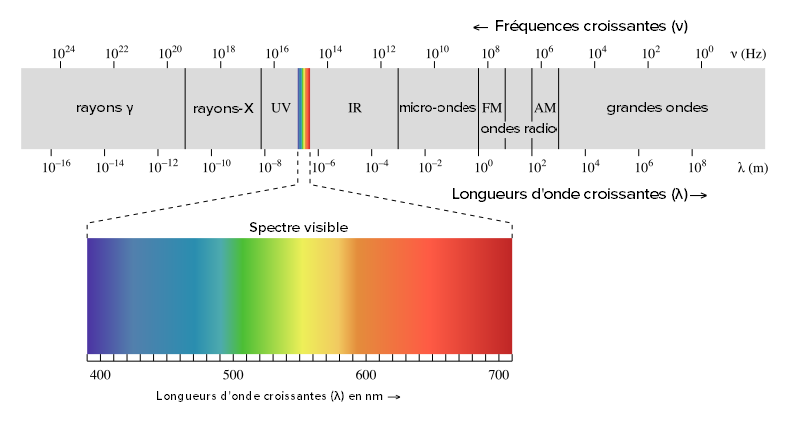
\includegraphics[width=0.9\textwidth]{images/spectre-electromagnetique.png}
    \caption{Spectre électromagnétique}
\end{figure}











\section{Les liaisons hertziennes en espace libre}
\subsection{Propagation dans l'environnement terrestre}
Il y a 4 types de d'ondes :
\begin{itemize}
  \item Les ondes de sol (ou de surface) : ces ondes suivent la courbure
  de la terre ($f$ = 3 KHz\ à\ 3 MHz), elles sont très stables mais une portée limitée (environ 500km).
  \item Les ondes de ciel : ces ondes sont réfléchies par les couches
  ionisées de l'atmosphère. L'onde pénétrant dans une de ces
  couches subit une réfraction qui peut devenir suffisante pour qu'il
  y ait réflexion. L'onde est alors renvoyée vers le sol.
  (portée mondiale, mais peut avoir des interférences avec l'onde de sol.) ($f$ = 3 MHz\ à\ 30 MHz)
  \item L'onde réfléchie : le sol conduit l'électricité et constitue un
  réflecteur des ondes radio ($f$ = 30 MHz\ à\ 3 GHz).
  \item L'onde directe : l'émetteur et le récepteur sont tout 2 "visibles l'un pour l'autre" ($f$ = 3 GHz\ à\ 30 GHz).
\end{itemize}

\begin{figure}[H]
  \centering
  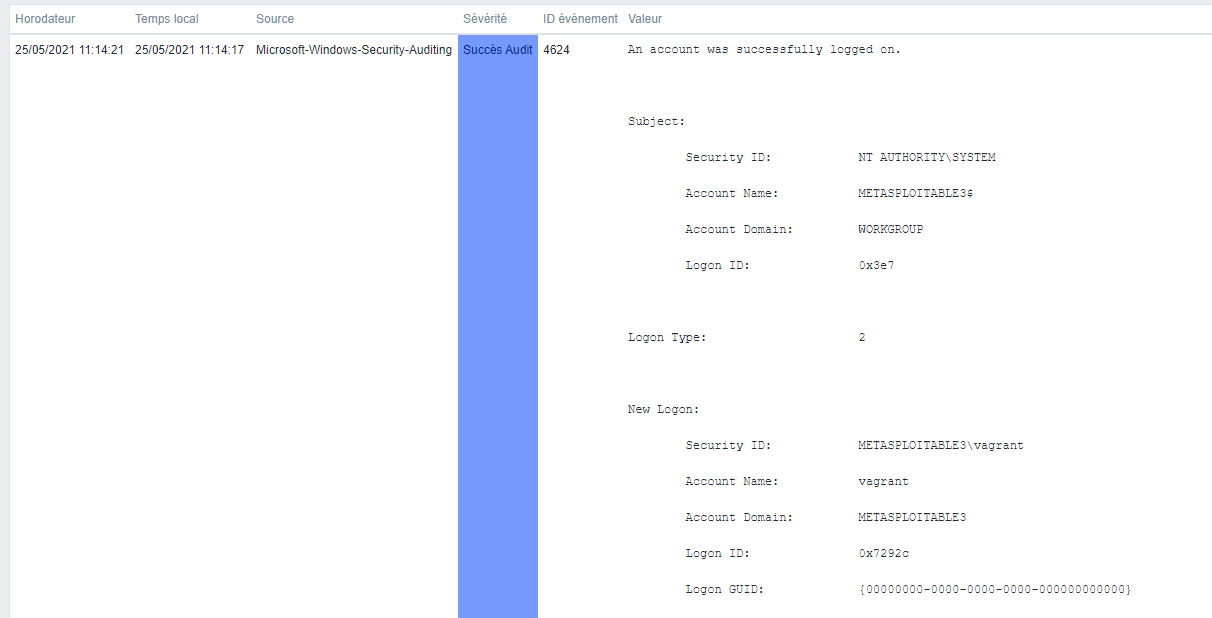
\includegraphics[width = 0.95\textwidth]{images/1.PNG}
  \caption{Schéma des différents types d'ondes}
\end{figure}

\subsection{Atténuation et absorption}
\subsubsection{Atténuation}

Plus une onde électromagnétique s'éloigne de sa source, plus son amplitude diminue.

\subsubsection{Absorption}

Dès qu'on quitte le vide, l'onde électromagnétique
va rencontrer des électrons qu'elle va exciter mais ce
processus ne s'effectue pas sans perte et le
rendement diminue donc.

\subsection{Ellipsoïde de Fresnel}
Quand un signal est réfléchi, il est déphasé de 180° \textbf{et} il parcourt un chemin plus long que le signal direct, ce qui provoque un déphasage supplémentaire. Ces 2 phénomènes sont observables ci-dessous
\begin{figure}[H]
  \centering
  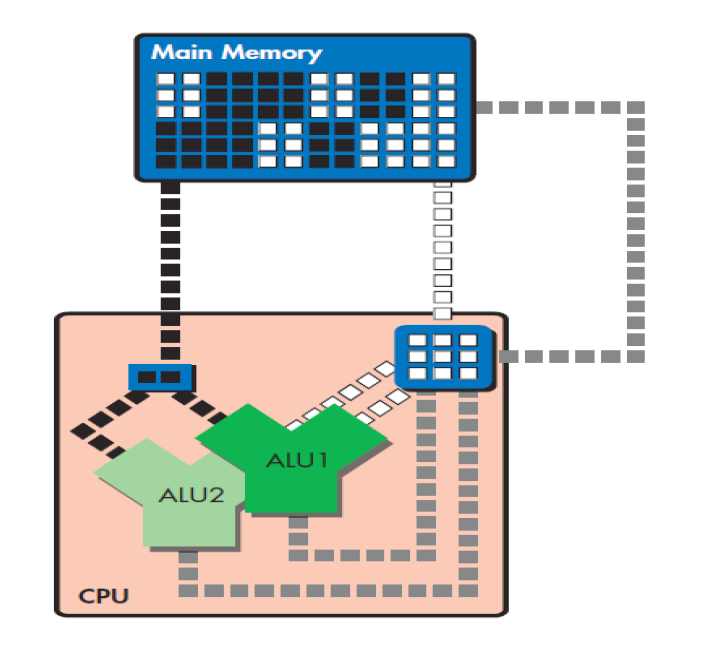
\includegraphics[width = 0.95\textwidth]{images/2.PNG}
  \caption{Phénomènes lors d'une réflexion}
\end{figure}

On calcule la zone de Fresnel de sorte qu'un signal qui y soit réfléchi et que le signal soit déphasé de 180°. 
Ainsi, le déphasage de 180° plus les 180° de la réflexion totalise 360° de déphasage, il n'y a donc pour ainsi dire "aucune modification" !

De plus, le premier ellipsoïde (zone) de Fresnel délimite la région où est
contenue la plus grande partie de l’énergie électromagnétique et donc si il n'y a pas d'obstacle dans cette zone à plus de 40\%, la propagation se fait en direct (donc par "visibilité").

Voici l'image illustrant la manière de calculer cette zone :
\begin{figure}[H]
  \centering
  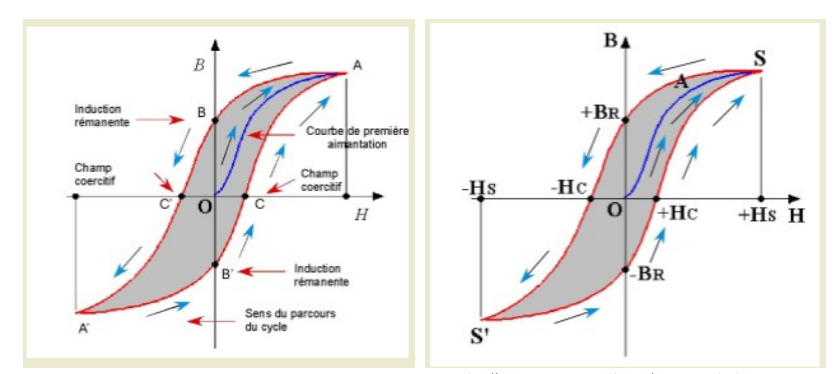
\includegraphics[width = 0.95\textwidth]{images/3.PNG}
  \caption{Calcul de la largeur de la Zone de Fresnel}
\end{figure}

Exemple :\\
À quelle hauteur doit on implanter deux tours hertziennes
séparées de 50km pour assurer une liaison en 10Ghz ?\\
La hauteur de végétation moyenne est de 15m !\\
Distance entre l'émetteur et le récepteur : 50km\\
Hauteur des obstacles : 15m\\
Comme on veut connaître la largeur maximale de la zone de Fresnel, on va calculer sa largeur a la moitié de la distance,
d1 et d2 sont alors égal a $\frac{50 \; km}{2}$.\\
$$ \lambda = \frac{3 \times 10^8}{10 \times 10^9} = 0,03m$$
$$ R_{max} = \frac{1}{2} \times \sqrt{0,03 \times 50000} = 19,4m $$
$$ D_{max} = 2 \times 19,4 = 38,8m $$
$$40\% D_{max} = 15,52m$$

Nous avons donc 15,52m qui peuvent se trouver dans les arbres !\\
Il restera 60\% pour être LOS. Les antennes peuvent donc simplement être à $R_{max}$, puis-ce que dans ce cas, il n'y a que 15m d'obstacle.

\subsection{Types de liaisons}
\begin{itemize}
  \item Liaison simplex : L'information ne va que dans un sens (émetteur $\rightarrow$ récepteur)
  \item Liaison half-duplex : L'information va dans les 2 sens mais pas en même temps
  \item Liaison duplex : L'information va dans les 2 sens et en même temps
\end{itemize}

\section{Les antennes}

\subsection{Le Décibel}

\begin{itemize}

\item Le nombre de décibels est donné par:
\[ 10 \log \frac{P_2}{P_1} = 20 \log \frac{V_2}{V_1} \]
où: P = puissance et V = tension.


\item Les différents types de dB:
\begin{itemize}
    \item dBW (= dB watt): $\displaystyle P_{dBW} = 10 \log \frac{P}{1 \; [W]} $
    \item dBm (dB miliwatt): $\displaystyle P_{dBm} = 10 \log \frac{P}{1 \; [mW]} $
    \item dBi (dB isotrope): gain d'une antenne par rapport à une antenne isotrope qui rayonnerait la même puissance dans toutes les directions.
\end{itemize}
Remarque: le gain de l'antenne traduit le fait que le rayonnement est favorisé dans certaines directions au détriment des autres. Il n'a physiquement rien à voir avec le gain d'un amplificateur.

\subsection{Caractéristiques des antennes}
L'antenne joue le rôle de transition entre le circuit électrique et le moyen de propagation.\\
En émission : un courant $\rightarrow$ un champ électromagnétique\\
En réception : un champ électromagnétique $\rightarrow$ un courant\\
\subsubsection{Évolution des ondes dans le spectre fréquentiel}
Plus la fréquence d'une onde sera basse, alors la distance de propagation et la taille de l'antenne seront plus importantes.\\
Plus la fréquence d'une onde est élevé, plus les antennes seront petite et la distance de propagation plus faible.

\subsection{Diagramme de rayonnement}
La directivité d'une antenne est une caractéristique très importante !
\begin{center}
   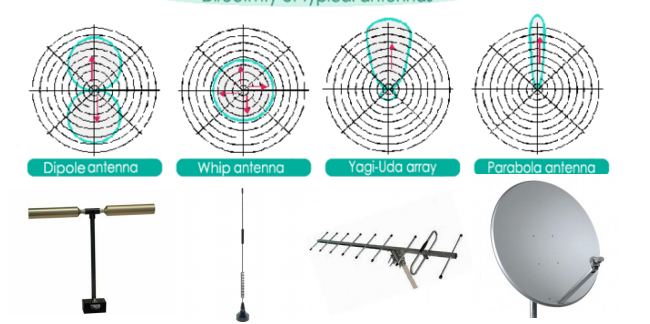
\includegraphics[width = 0.7 \textwidth]{images/4.PNG} 
\end{center}

L'angle d'ouverture d'une antenne est l'angle de direction pour lequel la puissance rayonnée est la moitié (-3 dB) de celle dans la direction la plus favorable.

\begin{center}
    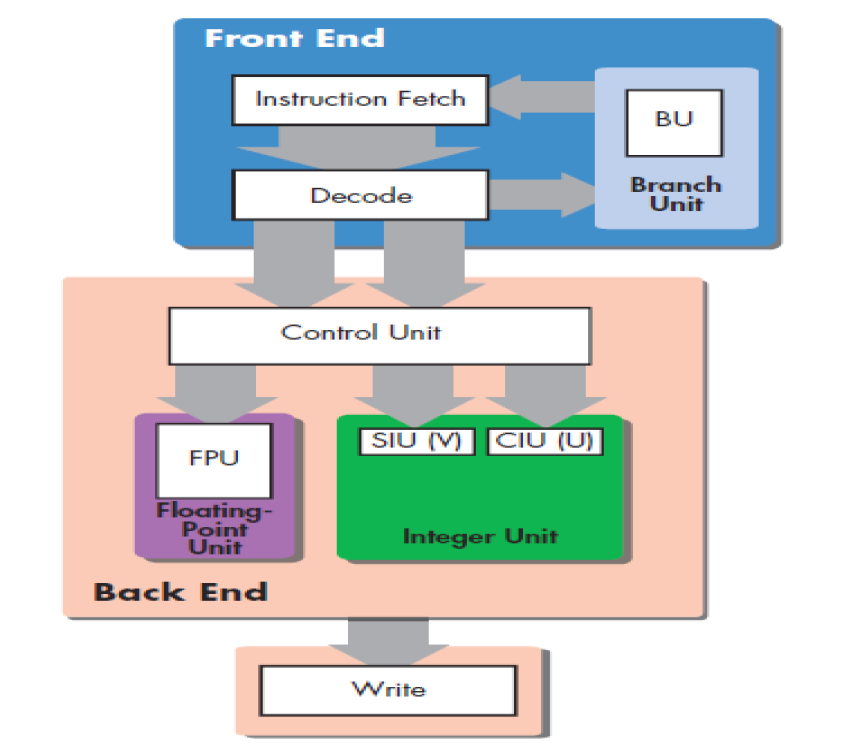
\includegraphics[width = 0.7 \textwidth]{images/5.PNG}
\end{center}

\subsection{Gain d'une antenne}
Pour bien comprendre, il faut bien faire l'analogie entre une antenne isotrope qui émet de la même \textbf{puissance} dans toutes les directions
et une antenne directive qui émet de la \textbf{puissance} que dans un certain angle.
\item Définition : Le gain de l'antenne est le fait de favoriser le rayonnement dans certaines directions au détriment des autres. Donc P0 étant la puissance d'une antenne isotrope et P1 étant la puissance d'une antenne
directive, le gain de l'antenne serait P1 - P0.
\item Gain d'une antenne d'angle $ < $ 90\textdegree:
\[ G_{\text{dBi}} = 10 \log \frac{41 \; 000}{\theta_H \; \theta_V} \]
où:
\begin{itemize}
    \item $ \theta_H $ = angle d'ouverture à l'horizontal (en degrés),
    \item $ \theta_V $ = angle d'ouverture à la verticale (en degrés),
    \item $ G $ = gain de l'antenne en dBi.
\end{itemize}

\subsection{Polarisation}

\item Le signal émis par une antenne est polarisé, c-à-d que le champ électrique est émis dans une certaine direction par rapport a l'horizontale. La référence étant toujours
la surface de la terre. Par exemple : Si le champ est parallèle à la surface de la terre alors la polarisation est linéaire horizontale.

\begin{center}
    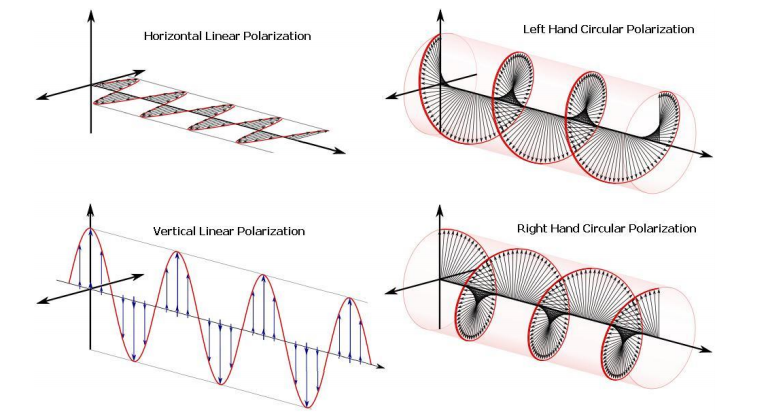
\includegraphics[width = 8cm]{images/6.PNG}
\end{center}

\subsection{Bande passante}

\item La bande passante d'une antenne est la bande de fréquence dans laquelle le champ rayonné est inférieur ou égal à 3dB en dessous du maximum.
\begin{center}
    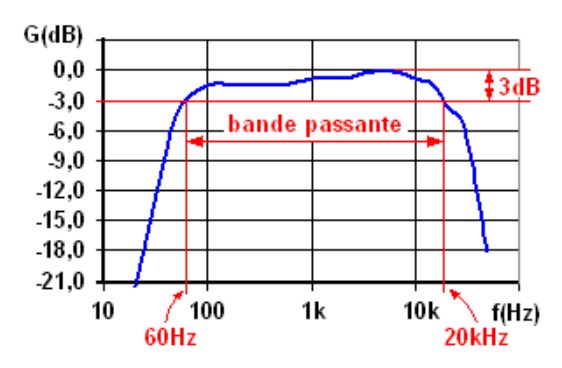
\includegraphics[width=0.5\textwidth]{images/bande-passante.PNG}
\end{center}


\end{itemize}



\section{Traitement des signaux}

\subsection{Signal et Bruit}

Définitions:
\begin{itemize}
    \item Un signal est la manifestation physique de l'information qu'il transporte de sa source à son destinataire.
    \item Le bruit est un phénomène perturbateur gênant la perception ou l'interprétation d'un signal.
    
\end{itemize}

\subsection{Signal sinusoïdal}

Expression du signal:
\begin{center}
    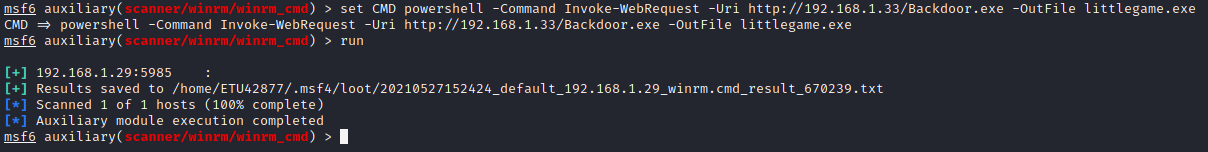
\includegraphics[width = 6cm]{images/7.PNG}
\end{center}
\[ x(t) = A \cos( \omega t + \phi) \]
où:
\begin{itemize}
    \item $ A $ est l'amplitude du signal,
    \item $ \omega $ est la pulsation du signal,
    \item $ \phi $ ou $ \varphi $ est la phase à l'origine.
\end{itemize}
Remarque: le signal "crête-crête" va du minimum au maximum ($= 2 \times A $).


La pulsation $ \omega $ est liée à la période et la fréquence par les relations suivantes:
\begin{itemize}
    \item $\displaystyle \omega = \frac{2 \pi}{T} $
    \item $ \omega = 2 \pi f $
\end{itemize}
Pour rappel: $\displaystyle T = \frac{1}{f} $

\subsection{Le déphasage}
Le déphasage ($ \Delta \phi $) est la différence de phase à l’origine des signaux étudiés.
\begin{center}
    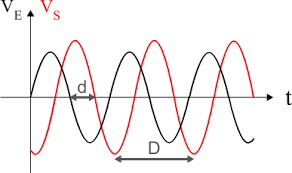
\includegraphics[width=0.4\textwidth]{images/dephasage.png}
\end{center}
\[ \Delta \phi = \frac{2 \pi d}{D} \]


\subsection{Série de Fourier}

Une série de Fourier est une série de fonctions sinusoïdales dont la somme permet de construire une fonction périodique déterminée de fréquence f.
\[ F_n = a_0 + \sum_{n = 1}^{\infty} a_n \cos(n x) + b_n \sin(n x) \]


\subsection{Spectre d'un signal}
Le Spectre d’un signal est la représentation fréquentielle des amplitudes du signal. On le représente en    
$ \frac{\text{Amplitude}}{\text{Fréquence}} $.
La théorie de Fourier permet de déterminer le spectre du signal.

\subsection{Utilité de traiter un signal}
\begin{itemize}
    \item Sans traitement, besoin d'antennes de dizaine de km
    \item Les hautes fréquences se propagent mieux dans l'air
    \item Le bruit peut être important
\end{itemize}

\section{Modulation analogique}
La modulation doit permettre à une puissante porteuse d’émettre
par voie aérienne les informations utiles.
Il y a 3 moyen de transmettre un message par l'onde porteuse :
\subsection{La modulation d'amplitude - AM}
L'amplitude de la porteuse varie linéairement en fonction de l'amplitude du message.\\
$Ac$ étant l'amplitude de la porteuse et $x(t)$ l'amplitude du message, on obtient notre signal en additionnant les 2 !
\begin{center}
    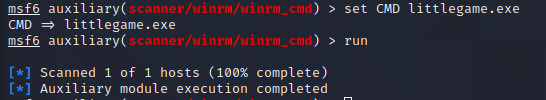
\includegraphics[width = 0.5 \textwidth]{images/8.PNG}
\end{center}

Expression du signal :
$$ V_{AM} (t) = (A_c + x(t)) \times cos(\omega_c  \times t + \Phi_c) $$
Le \emph{Taux de modulation} est le rapport entre la modulation du signal obtenu et la modulation de la porteuse. On la représente ainsi : $$ m = \frac{\text{Amplitude Signal Modulé (Am)}}{\text{Amplitude de la porteuse (Ac)}} $$

Si $x(t)$ > $Ac$, alors ils y a \emph{surmodulation} !\\
Il y a 2 types de modulation d'amplitude :
\begin{itemize}
    \item Double Size Band (DSB) : Les 2 bandes latérales du signal modulé sont transmises, la porteuse n'est pas transmise.
    \item Single Size Band (SSB) : Une seule des 2 bandes latérales du signal modulé est transmise, la porteuse n'est pas transmise. (occupation spectrale beaucoup moins importante)
\end{itemize}

\subsubsection{Démodulation d'amplitude}
On veut retrouver le message a partir du signal modulé. Il y a 2 moyens :
\begin{itemize}
    \item Démodulation synchrone : Multiplication du signal modulé par un signal sinusoïdal en phase avec la porteuse.
    \item Démodulation d'enveloppe : Grâce a une diode qui laissera le courant passer que dans un sens, on garde la partie positive du signal et on observe l'enveloppe du signal.
\end{itemize}

\subsection{Modulation de fréquence - FM}
Le signal obtenu gardera une puissance/une amplitude constante mais sa fréquence variera selon l'amplitude du message !
\begin{center}
    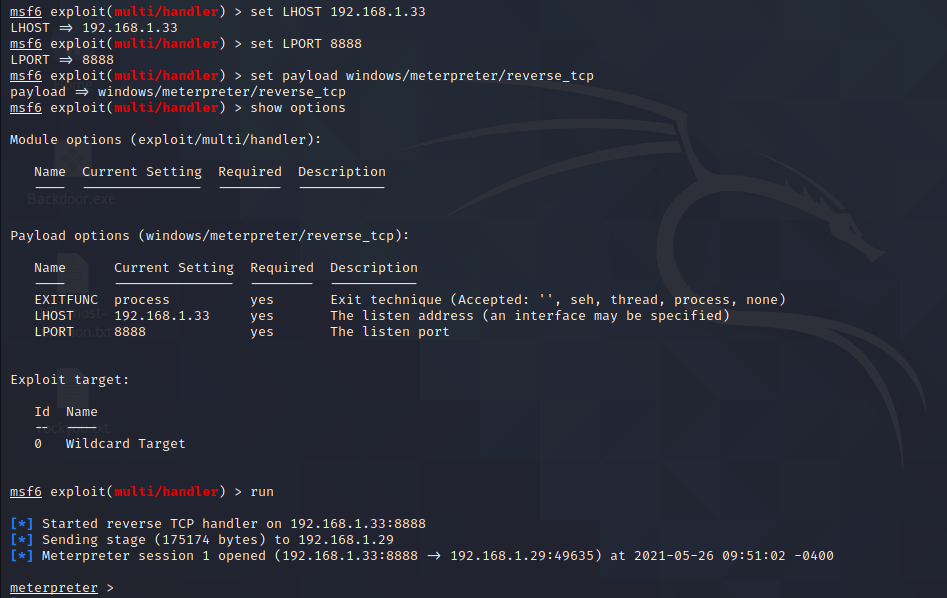
\includegraphics[width = 0.8 \textwidth]{images/9.PNG}
\end{center}

Expression du signal modulé : 
$$ V_{FM}(t) = A_c \times cos(\omega_c \times t + m \times sin(\omega_m \times t)) $$

Plus la tension du message augmente (amplitude), plus la fréquence du signal modulé augmente ! 
Au contraire, plus la tension du message diminue, plus la fréquence du signal diminue !

Avantages :
\begin{itemize}
    \item Puissance constante
    \item Moins de sensibilité au bruit
    \item Pas de sur-modulation
\end{itemize}

Inconvénient :
\begin{itemize}
    \item Largeur de bande plus importante qu'en modulation d'amplitude
\end{itemize}
Fréquence instantanée de la porteuse :
$$ f_i = f_c + k \times x(t) $$
\begin{itemize}
    \item $f_c$ étant la fréquence de la porteuse
    \item $x(t)$ étant le signal à transmettre
    \item $k$ est une constante
\end{itemize}

L'excursion de fréquence $\Delta f$ = la variation maximale de la fréquence du signal modulé par rapport au signal de la porteuse.

L'indice de modulation : 
$$ m = \frac{\Delta f}{f_M} $$
\begin{itemize}
    \item $\Delta f$ étant l'excursion de fréquence
    \item $f_M$ étant la fréquence du signal modulant
\end{itemize}

Contrairement à \emph{AM}, le spectre \emph{FM} ne se calcule qu'en basse fréquence !

\subsection{Modulation de phase - PM}
Le message est transmis par les variations de phase instantanée d'une onde porteuse.
Modulation est peu utilisée !

Expression du signal modulé :
$$ V_{PM}(t) = A_c \times cos(\omega_c \times t + k \times x(t))$$

La modulation de phase est semblable a la modulation de fréquence.\\ Elle est en avance par rapport a la FM d'un quart de période soit 90°.
\begin{center}
    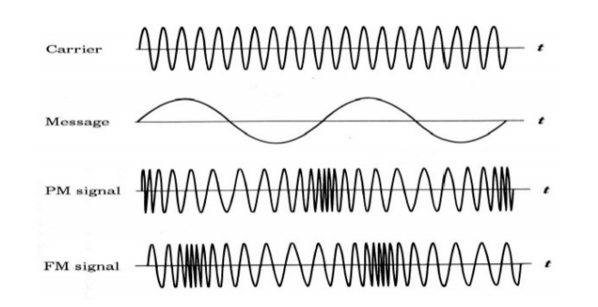
\includegraphics[width = 0.8 \textwidth]{images/10.png}
\end{center}

\section{La modulation numérique}

\subsection{Transmissions numérique en bande de base}
$$Informations\ \rightarrow\ Signaux numeriques$$\\
Débit binaire :
\begin{itemize}
    \item Les bits sont émis au rythme d'un signal d'horloge
    \item Le débit binaire est le nombre de bits transmis par seconde
\end{itemize}

Exemples :
\begin{itemize}
    \item $NRZ \rightarrow RS232$
    \item $NRZ-I \rightarrow USB$
    \item $Manchester \rightarrow Ethernet$
\end{itemize}

\subsubsection{Codage NRZ bipolaire}
NRZ = Non return to zero\\
$0 \Rightarrow -a$\\
$1 \Rightarrow +a$\\

\begin{center}
    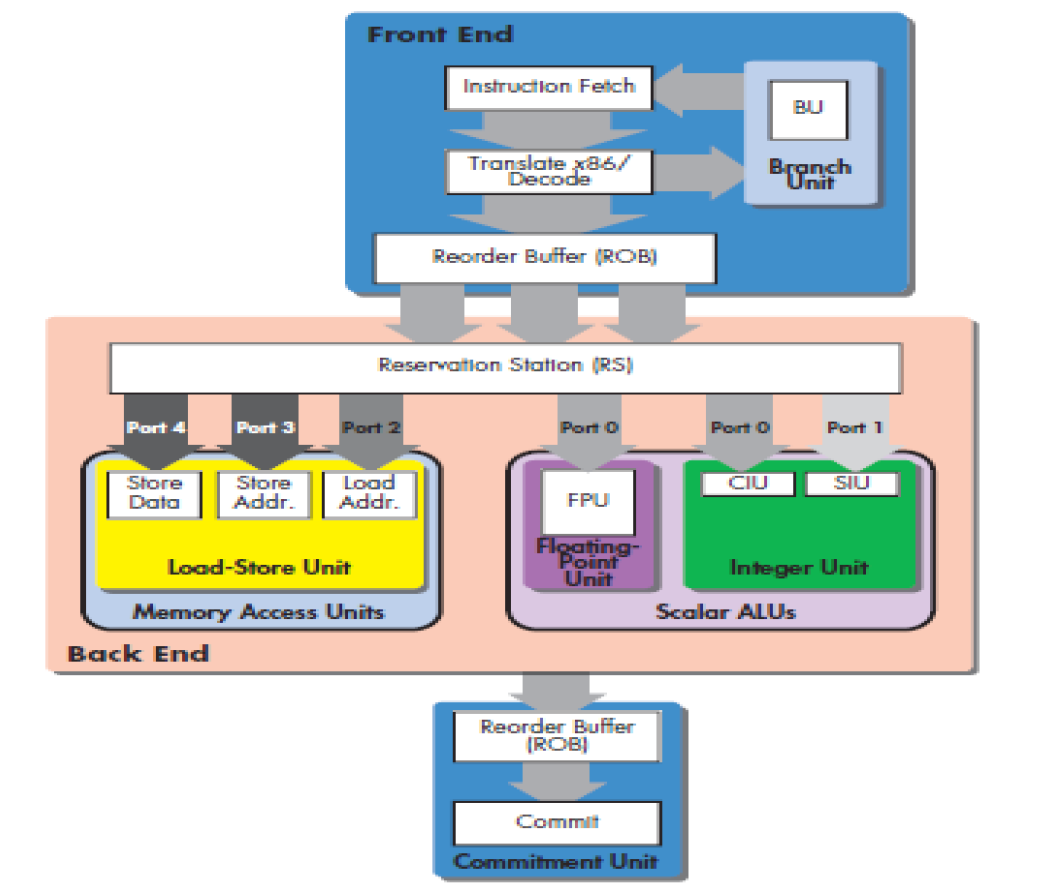
\includegraphics[width = 0.8 \textwidth]{images/11.PNG}
\end{center}

\subsubsection{Codage NRZ unipolaire}
NRZ = Non return to zero\\
$0\Rightarrow 0V$\\
$1 \Rightarrow +a$

\subsubsection{Codage NRZ-I}
NRZ-I = Non return to zero inverted\\
$0 \Rightarrow$ même état que l'état précédent\\
$1 \Rightarrow$ transition\\
Une suite de 0 est difficile a compter

\begin{center}
    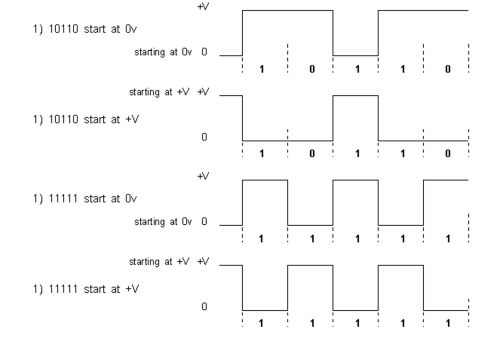
\includegraphics[width = 0.8 \textwidth]{images/12.PNG}
\end{center}

\subsubsection{Codage RZ}
RZ = Return to zero\\
$1 \Rightarrow$ retourne a 0 pendant la 2ème moitié du bit
\begin{center}
    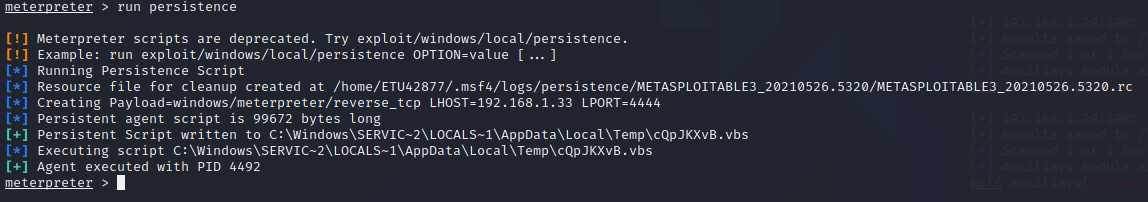
\includegraphics[width = 0.8 \textwidth]{images/13.PNG}
\end{center}

\subsubsection{Codage Manchester}
\begin{itemize}
    \item Permet de décaler le spectre du signal vers les fréquences plus élevées
    \item Code par les états de bases des transitions
    \item $1 \Rightarrow$ front descendant
    \item $0 \Rightarrow$ front montant
    \item Facilité de synchronisation d'horloge car + de transitions
\end{itemize}
\begin{center}
    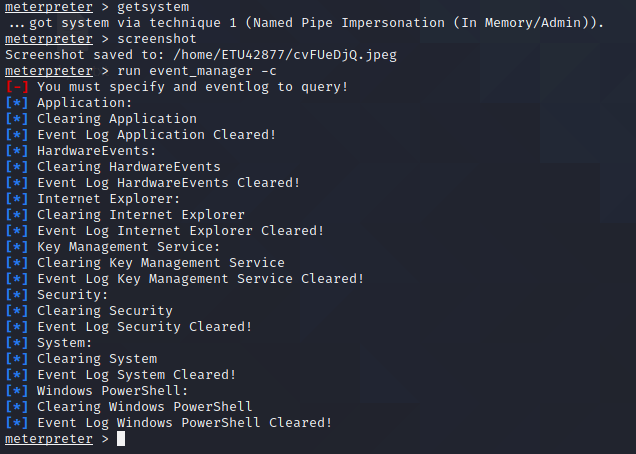
\includegraphics[width = 0.8 \textwidth]{images/14.PNG}
\end{center}

\subsection{Codes détecteurs et correcteurs d'erreurs}

\subsubsection{Détection d'erreur : bit de parité}
\begin{itemize}
    \item Ajout d'un bit a chaque octet
    \item Si un bit est faux, pas de correction mais demande de répétition
    \item Si 2 bits sont faux, pas de détection
    \item Si bit de parité erroné, répétition alors qu'il n'y a pas d'erreur
\end{itemize}

\subsubsection{Correcteurs d'erreurs}
\begin{itemize}
    \item Permet de détecter et corriger les erreurs
    \item Exemple : Code de Hamming (vu en Logique/Numération)
\end{itemize}

\subsubsection{Entrelacement}
L'entrelacement modifie l'ordre des données de façon a ce qu'une suite d'erreurs consécutives soient transformées en erreurs isolées après le désentrelacement.

Exemple :
\begin{center}
    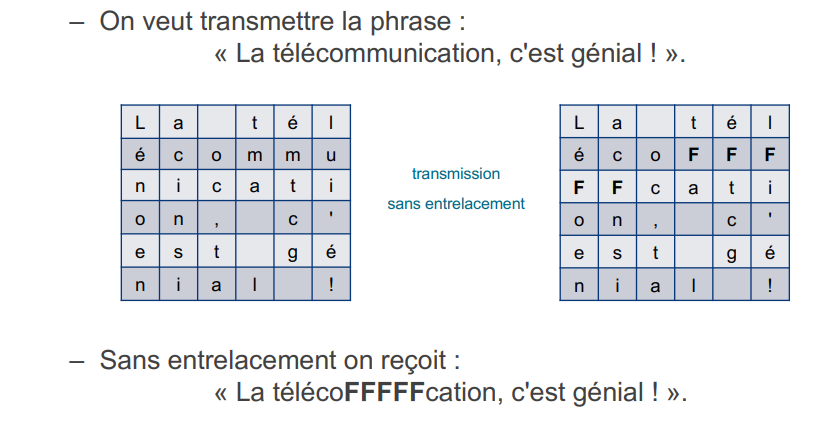
\includegraphics[width = 0.5 \textwidth]{images/15.PNG}
    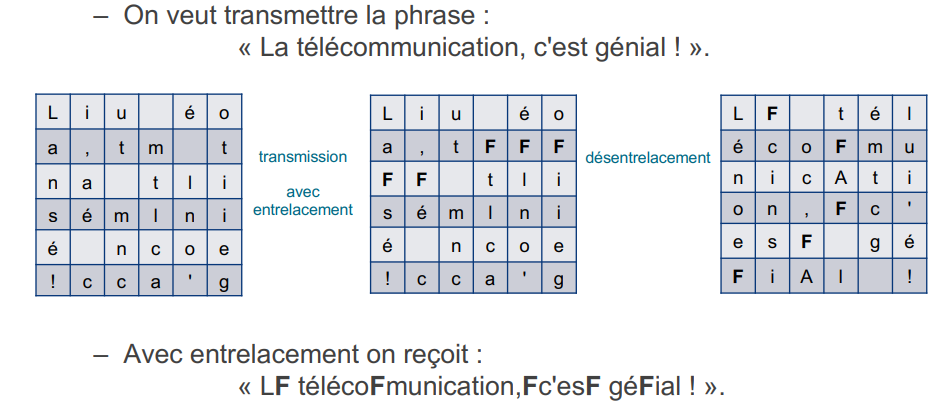
\includegraphics[width = 0.5 \textwidth]{images/16.PNG}
\end{center}

\subsection{Modulation ASK}
\begin{itemize}
    \item ASK $\rightarrow$ Amplitude Shift Keying
    \item Modulation numérique de l'amplitude
    \item Équivalent à la AM
    \item Le signal à transmettre n'est plus analogique mais par exemple un signal NRZ. Consiste à transmettre un signal sinusoïdal de la fréquence de la porteuse $f_c$ et d'amplitude $A_0$ au bit 0 et une amplitude $A_1$ au bit 1.
    \item Peu utilisé si > Mbit/s et pas plus d'une dizaine de mètres
\end{itemize}

\subsection{Modulation FSK}
\begin{itemize}
    \item FSK $\rightarrow$ Frequency Shift Keying
    \item Modulation Numérique de la Fréquence
    \item Équivalent à la FM
    \item Le signal à transmettre n'est plus analogique mais par exemple un signal NRZ. 
Consiste à transmettre un signal sinusoïdal d’amplitude constante et de fréquence $f_0$ au bit 0 et une fréquence $f_1$ au bit 1.
\end{itemize}
\subsubsection{Modulation 4FSK}
C'est une variante de FSK !\\
\begin{itemize}
    \item Permet une modulation à 4 états de fréquence au lieu de 2
    \item Permet de diviser l'occupation su spectre par 2 en regroupant les bits a transmettre 2 par 2.
\end{itemize}
\subsubsection{Modulation AFSK - Audio FSK}
\begin{itemize}
    \item La porteuse est un signal audible
    \item Ne permet pas de débit rapide
\end{itemize}
\subsection{Modulation PSK}
\begin{itemize}
    \item PSK ou BPSK $\rightarrow$ Binary Phase Shift Keying
    \item Modulation Numérique de Phase
    \item Équivalent à la PM
    \item Le signal à transmettre n'est plus analogique mais par exemple un signal NRZ. 
Consiste à transmettre un signal sinusoïdal d’amplitude constante dont l’expression est $A.cos(\omega c.t+ \phi_0)$ au bit 0 et une fréquence $A.cos(\omega c.t+ \phi_1)$ au bit 1.
    \item En général $\phi_1 - \phi_2 = \pi (180$°$)$
    
\end{itemize}
\subsection{Modulation QPSK}
\begin{itemize}
    \item QPSK $\rightarrow$ Quadrature Phase Shift Keying
    \item 2 porteuses déphasées de $\frac{\pi}{2}$ sont utilisés
    \item Porteuse de référence appelé "I", l'autre "Q"
    \item Les 2 porteuses sont codées séparément en BPSK et additionées pour obtenir le QPSK $\Rightarrow$ $ \pm sin(2\pi f_0 t) \pm cos(2 \pi f_0 t)$. Si on additionne, alors le bit est égal a 1, au contraire si on soustrait le bit sera égal a 0.\\ 
    Exemple : 1 0 (1 sur le canal I et 0 sur le canal Q) → $+sin(2\pi f_0 t)-cos(2\pi f_0 t)$
    \item Résistant au bruit (\textbf{IMPORTANT} il peut être intéressant de voir la constellation QPSK qui n'est pas abordée dans cette synthèse car très schématique)
\end{itemize}
\subsection{La modulation à plus de 4 états}
\subsubsection{Modulation 8PSK}
\begin{itemize}
    \item Bits regroupés pas 3
    \item Si erreur de codage, un seul bit sera concerné donc plus facile a corriger car 2 points adjacents sur la constellation ne diffèrent que d'un bit.
\end{itemize}

\subsubsection{Modulation 8QAM}
\begin{itemize}
    \item Combinaison de la modulation ASK et PSK
    \item Bits regroupés par 3, donc 8 combinaisons différents : $2^3 = 8$
\end{itemize}









\section{La modulation d'impulsions analogiques} %% début = slide 156



Il y en a 4:
\begin{itemize}
    \item PAM = Pulse Amplitude Modulation
    \item PWM = Pulse Width Modulation
    \item PPM = Pulse Position Modulation
    \item PCM = Pulse Coded Modulation
\end{itemize}
\begin{center}
    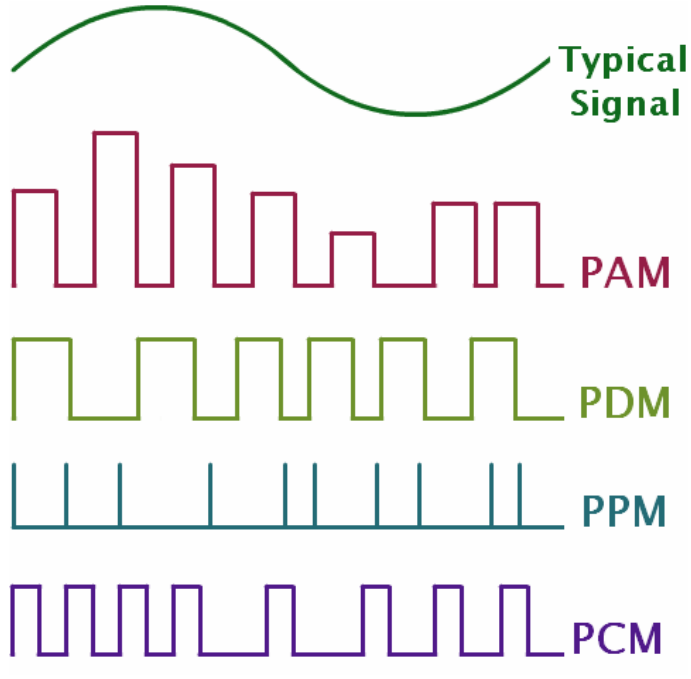
\includegraphics[width=0.5\textwidth]{images/mod-impulsions-analog-01.PNG}
\end{center}





\subsection{Pulse Amplitude Modulation}



La PAM (ou Modulation d’impulsion par l’amplitude) est un type de modulation impulsionnel dont le principe est de donner à un train d’impulsion l’amplitude du signal à transmettre. Le train d’impulsions est à fréquence fixe.
\begin{center}
    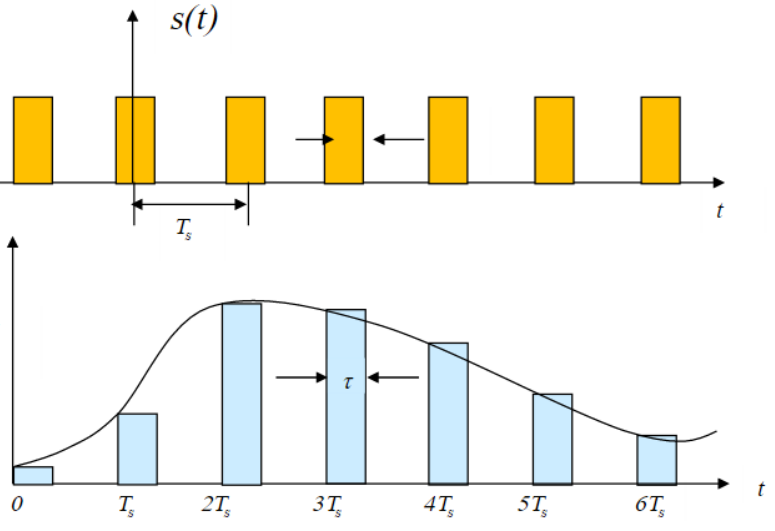
\includegraphics[width=0.5\textwidth]{images/PAM-01.PNG}
\end{center}





\subsection{Pulse Width Modulation}



La PWM (modulation par largeur d’impulsion) est une technique de modulation impulsionnelle qui consiste à garder l’amplitude du signal impulsionnel constante et qui fait varier sa largeur d’impulsion tout en gardant la fréquence constante. La génération d'un signal PWM est facile à mettre en œuvre et c'est une technique très utilisée.
\begin{center}
    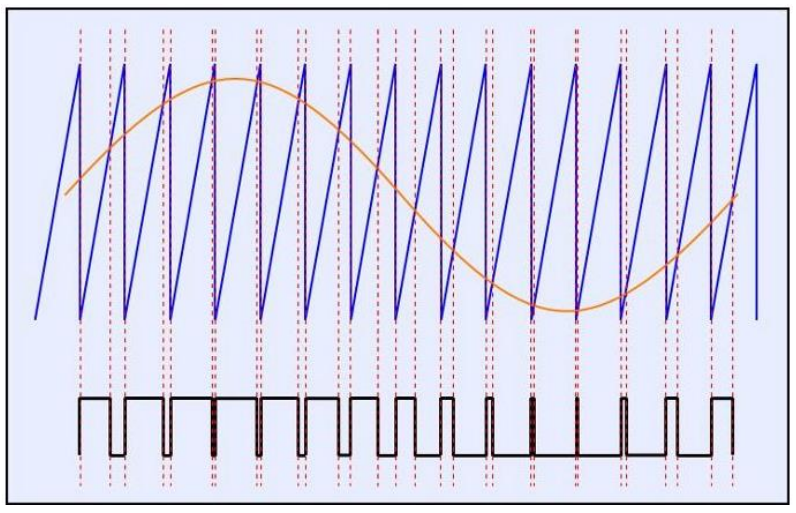
\includegraphics[width=0.5\textwidth]{images/PWM-01.PNG}
\end{center}





\subsection{Pulse Position Modulation}



\subsubsection{PPM normale}

Cette technique de modulation impulsionnelle consiste à garder l’amplitude du signal impulsionnel constant en faisant varier la position d’une impulsion de largeur fixe tout en gardant la fréquence constante. Les 0 et 1 sont convertis en durée entre l'horloge et les
impulsions:
\begin{itemize}
    \item Une petite durée représente un 0 numérique.
    \item Une grande durée représente un 1 numérique.
\end{itemize}
\begin{center}
    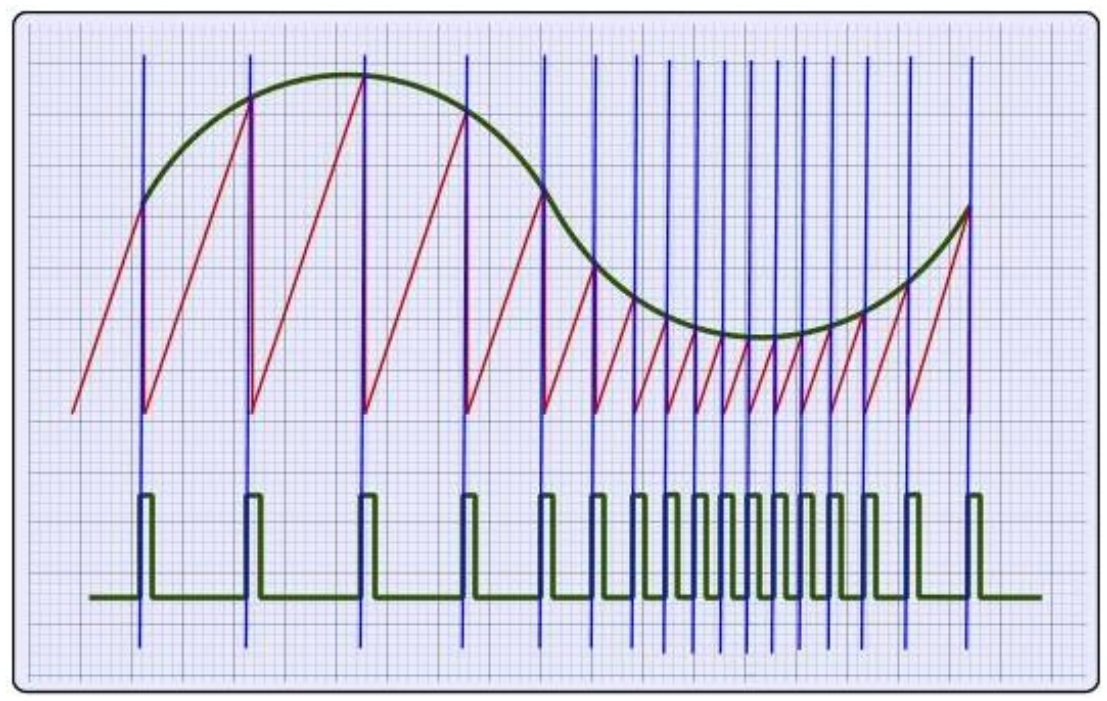
\includegraphics[width=0.5\textwidth]{images/PPM-01.PNG}
\end{center}
Cette méthode a un grand désavantage. Le décodage du signal exige que le décodeur dispose d'une horloge parfaitement synchronisée avec l'émetteur.



\subsubsection{PPM différentielle}

La PPM différentielle est une variante de la modulation PPM. Elle permet la transmission des données indépendamment d'une horloge. Le délai entre les impulsions est calculé à partir du front descendant de l'impulsion précédente.
\begin{center}
    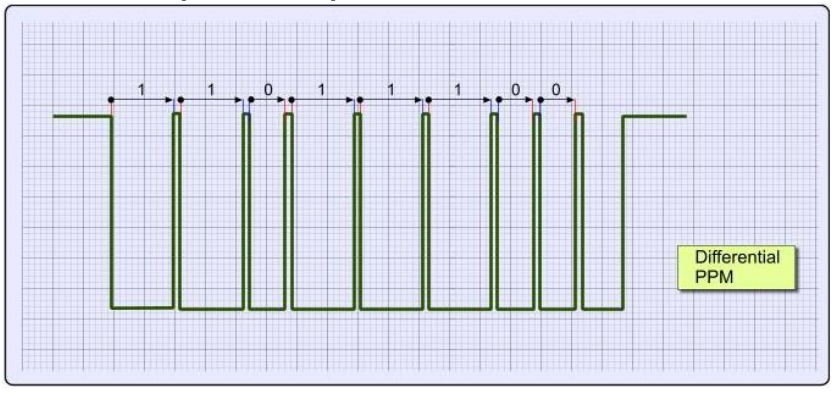
\includegraphics[width=0.5\textwidth]{images/PPM-02.PNG}
\end{center}
Contrairement à la PPM simple, la longueur du signal codé n'est pas fixé en PPM différentiel. La bande passante est donc plus élevée.





\subsection{Pulse Coded Modulation}



La PCM ou MIC (modulation par codage d'impulsion) est une conversion analogique-numérique dont le message est représenté par des mots binaires. Chaque mot possible correspond à une certaine valeur de l'amplitude du signal d'information.
\begin{center}
    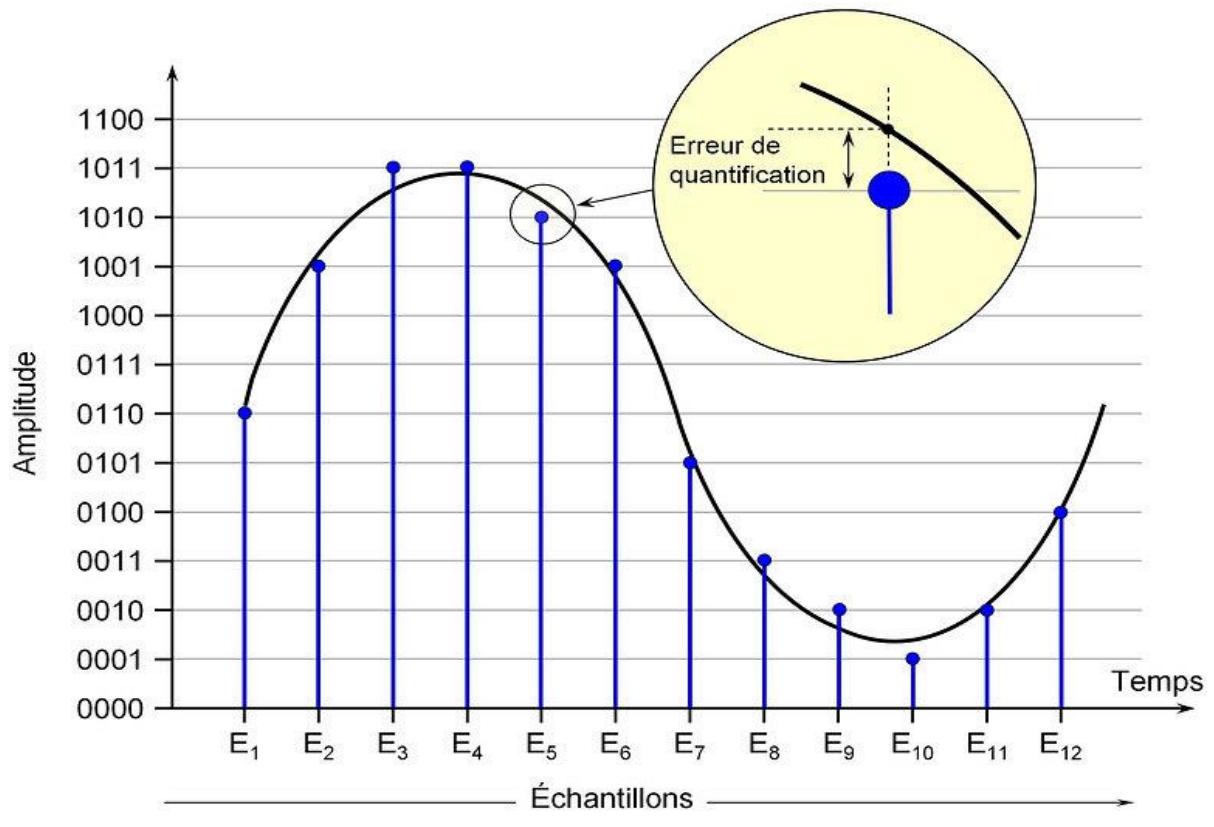
\includegraphics[width=0.65\textwidth]{images/PCM-03.PNG}
\end{center}
Toutes les valeurs analogiques ne peuvent pas être représentées ce qui implique une certaine erreur de quantification. Pour minimiser ces erreurs, on utilise le principe de compression du signal via une caractéristique logarithmique. Les petites amplitudes du signal sont quantifiées avec beaucoup plus de précision que les amplitudes élevées.
\begin{center}
    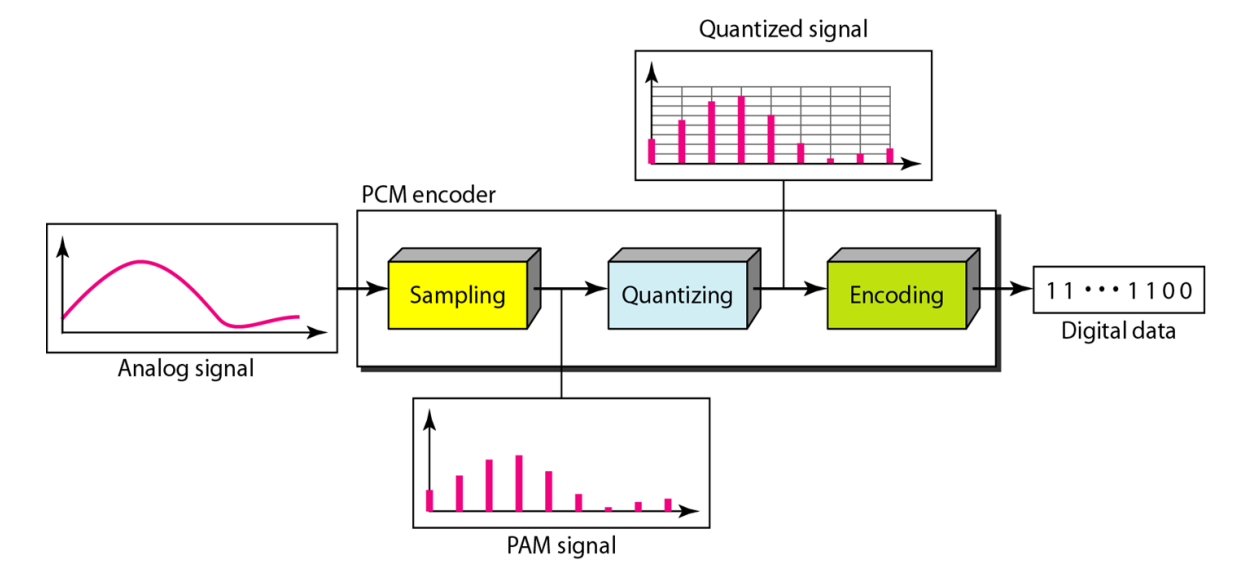
\includegraphics[width=0.85\textwidth]{images/PCM-02.PNG}
\end{center}
Comme on peut le voir sur le schéma, on commence en modulant le signal analogique en générant le signal PAM (modulation d'amplitude) puis on quantifie le signal et on l'encode (ce qui donne le signal final, la PCM).










\section{La fibre optique} %% début = slide 173





\subsection{Structure}



\begin{center}
    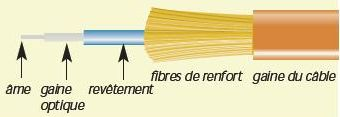
\includegraphics[width=0.5\textwidth]{images/fibre-01.JPG}
\end{center}
\begin{itemize}
    \item La gaine du câble protège contre l'usure, les solvants, ...
    \item Les fibres de renfort protègent l’âme contre l’écrasement et les tensions excessives.
    \item Le revêtement est une couche de plastique qui renforce l’âme, absorbe les chocs et offre une protection supplémentaire contre les courbures excessives du câble.
    \item La gaine optique est une fine couche qui sert de barrière pour retenir les ondes lumineuses et provoquer la réfraction.
    \item L'âme est le support physique qui transporte les signaux optiques entre une source de lumière et un équipement récepteur.
\end{itemize}





\subsection{Les différentes fibres optiques} %% début = slide 182



\begin{enumerate}
    \item La fibre optique \textbf{multi-mode à saut d'indice}: Le phénomène de réflexion totale va guider la lumière à se propager à l'intérieur du cœur de la fibre. Le guidage se fait donc en dent de scie.
    \item La fibre optique \textbf{multi-mode à gradient d'indice}:
    \begin{itemize}
        \item Dans une fibre optique à gradient d'indice, le faisceaux lumineux est continûment dévié vers l’axe optique de la fibre par un effet de focalisation.
        \item En subissant ces légères réfraction à l'approche de la gaine le signal optique forme un signal sinusoïdal (en hélice).
    \end{itemize}
    \item La fibre optique \textbf{mono-mode}:
    \begin{itemize}
        \item Elle a la particularité d'avoir un cœur avec un diamètre beaucoup plus petit.
        \item En théorie, le signal lumineux se déplace donc en ligne droite. En pratique, il se propage au voisinage de l'axe horizontal.
        \item Le taux d'atténuation est très faible car il n'y a pas de réfraction
    \end{itemize}
\end{enumerate}
\begin{center}
    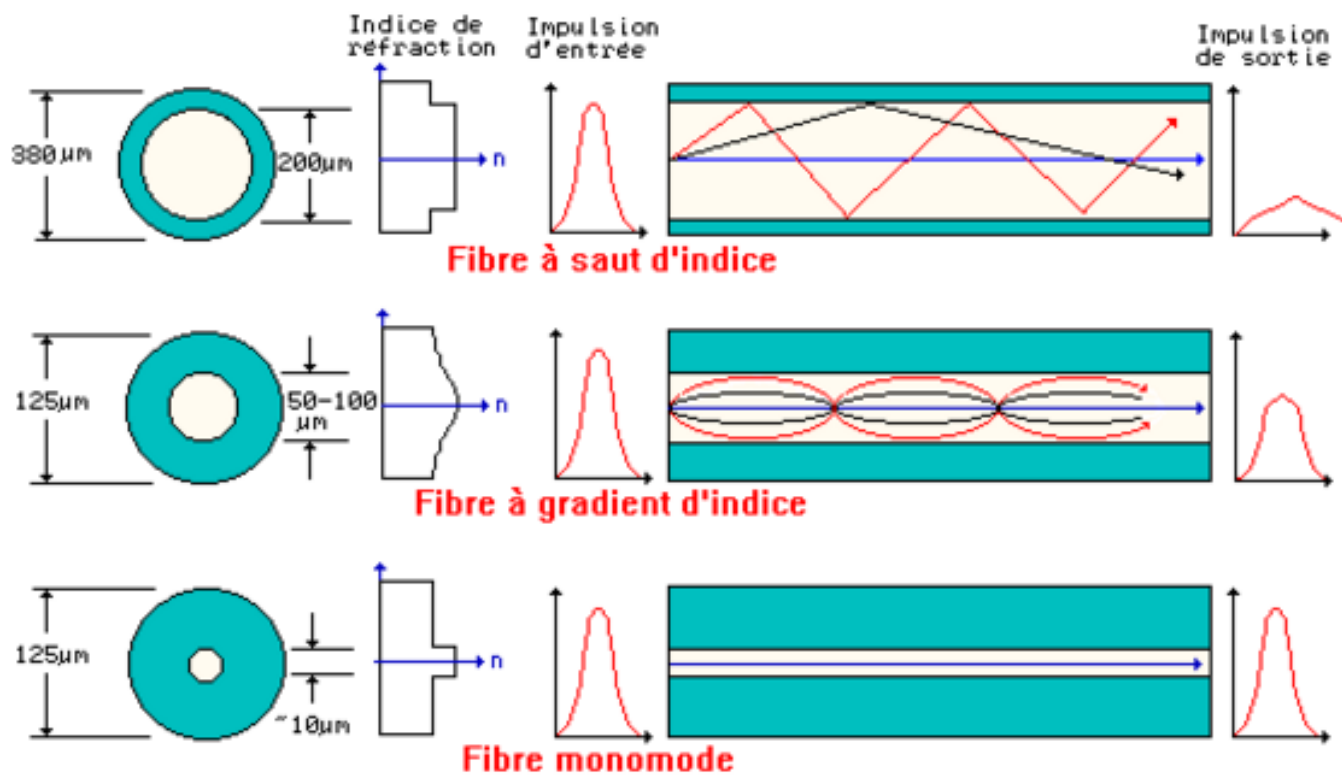
\includegraphics[width=0.65\textwidth]{images/fibre-04.PNG}
\end{center}





\subsection{Émetteurs optiques} %% début = slide 184



\begin{enumerate}
    \item Les LED:
    \begin{itemize}
        \item uniquement utilisées en fibres multimodes,
        \item peu chères, faciles à utiliser, moins rapides et faisceau plus large,
        \item procurent une moindre bande passante que les lasers et peuvent atteindre un débit maximal de 1 Gbit/s.
    \end{itemize}
    \item Les diodes laser:
    \begin{itemize}
        \item s’utilisent sur fibre monomode ou multimode,
        \item plus chères et plus rapides, faisceau plus étroit,
        \item peuvent atteindre un débit de 10 Gbits/s et plus.
    \end{itemize}
\end{enumerate}





\subsection{Détecteurs optiques}



\begin{itemize}
    \item Un détecteur optique converti les photons en courant électrique.
    \item Ce type de dispositif porte le nom de photodiode ou photo-détecteur.
\end{itemize}





\subsection{Modulations et multiplexages}



La modulation directe d'un laser: on module directement le courant injecté en entrée de la diode. A la suite de cette modulation de courant, l'intensité de la lumière produite par la diode sera affectée. Cette technique est moins onéreuse, mais présente des pertes et un facteur de bruit importants.

Le multiplexage: consiste à faire passer plusieurs informations sur un seul support de transmission.
\begin{itemize}
    \item TDM (= Time Division Multiplexing): consiste à affecter à un utilisateur unique la totalité de la bande passante pendant un court instant et à tour de rôle pour chaque utilisateur. Débit maximum de 5 Gb/s par modulation directe ou de 40 Gb/s par modulation externe.
    \item WDM (= Wavelength Division Multiplexing): les signaux sont portés par des longueurs d'ondes différentes, et espacées assez largement afin de ne pas interférer les unes avec les autres. Sur 1 canal (1 longueur d'onde) on atteint un débit de 5 Gb/s par modulation directe de la source ou de 40 Gb/s par modulation externe. Théoriquement, on pourrait obtenir 5 Tb/s en utilisant 125 canaux à 40 Gb/s.
    \begin{center}
        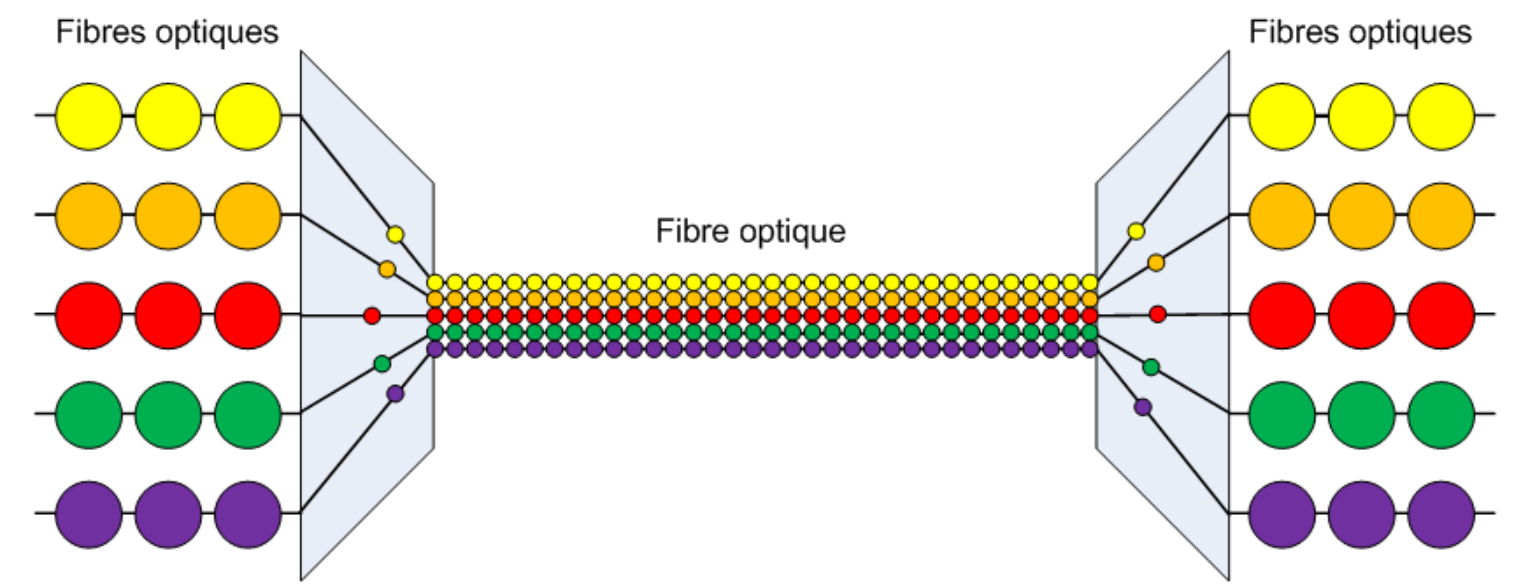
\includegraphics[width=0.75\textwidth]{images/fibre-05.PNG}
    \end{center}
    \item TDM / WDM: Les systèmes modernes de télécommunications optiques associent ces deux techniques pour atteindre les très hauts débits.
\end{itemize}

Bilan de liaison:
\begin{itemize}
    \item Différentes longueurs d'onde sont multiplexées sur une fibre de type monomode.
    \item Le signal est amplifié tous les 100 Km.
    \item Le démultiplexeur sépare les différentes longueur d'onde.
\end{itemize}










% \section{Courants porteurs en ligne} %% début = slide 196





% \subsection{Introduction}



% \begin{itemize}
%     \item CPL = Courants Porteurs en Ligne =  technique qui utilise le réseau d’énergie électrique pour transmettre tous les services de télécommunication.
%     \item On fait passer l'information avec des techniques de modulation.
% \end{itemize}





% \subsection{Support physique}



% \begin{itemize}
%     \item Pour la technologie CPL, le câble électrique fait office de support de la transmission des données (couche physique du modèle OSI).
%     \item Voici les différents types de bruits qui peuvent être perçus sur et autour du câble électrique:
%     \begin{itemize}
%         \item bruits impulsionnels dus aux arrêts et démarrages des appareils électriques
%         \item bruits blancs à large bande, dont la densité spectrale de puissance est la même pour toutes les fréquences
%         \item bruits harmoniques, composés des multiples fréquences utilisées par les équipements électriques branchés sur le réseau et qui sont, par exemple, des multiples de 50 Hz.
%     \end{itemize}
% \end{itemize}





% \subsection{Technologie}



% \begin{itemize}
%     \item Au signal électrique de 50 Hz on superpose un autre signal à plus haute fréquence (bande 1,6 à 30 MHz) et de faible énergie (<0,5V).
%     \begin{center}
%         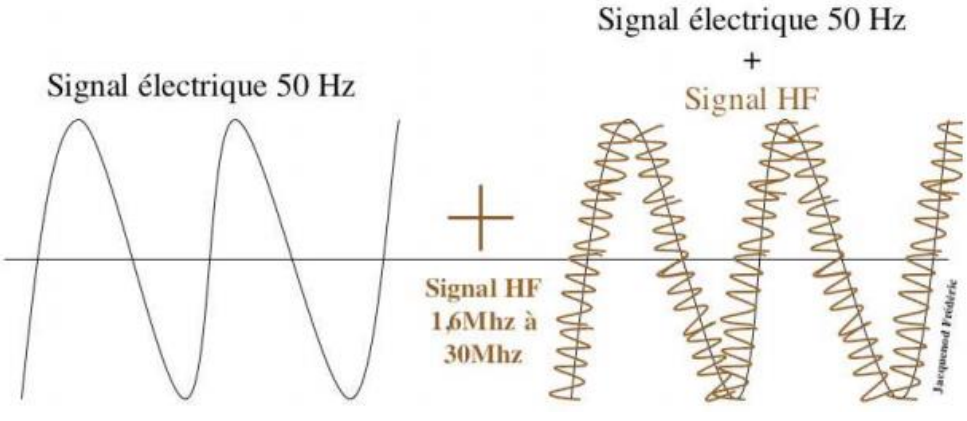
\includegraphics[width=0.5\textwidth]{images/CPL-1.PNG}
%     \end{center}
%     \item Ce deuxième signal se propage sur l'installation électrique et peut être reçu et décodé à distance.
%     \item Les adaptateurs CPL:
%     \begin{itemize}
%         \item Suppriment les basses fréquences (le courant)
%         \item Traitent le signal
%         \item Récupèrent le signal
%         \item Isolent les fréquences pour récupérer les données numériques
%     \end{itemize}
% \end{itemize}





% \subsection{Modulations}



% \begin{itemize}
%     \item Modulation OFDM = Orthogonal Frequency Division Multiplexing.
%     \item Le signal est réparti sur un grand nombre de sous-porteuses de fréquence distincte et ce dans plusieurs bandes de fréquences.
%     \item Une modulation monoporteuse réalise un multiplexage temporel, tandis qu'une modulation multiporteuses réalise un multiplexage fréquentiel.
%     \item La transformée de Fourier rapide inverse (IFFT) est un moyen facile pour moduler les données sur les sous-porteuses orthogonales.
%     \item Une des modulations à étalement de spectre est le CDMA (= code division multiple access). Il permet à plusieurs liaisons numériques d'utiliser simultanément la même fréquence porteuse.
%     \item Chaque liaison utilise son propre code. À la réception, le signal est perçu comme du bruit si le récepteur n'a pas le code. Cette modulation est ainsi optimisée pour lutter contre le bruit.
% \end{itemize}





% \subsection{Architectures}


% \begin{itemize}
%     \item Le CPL Indoor est une solution pour étendre le réseau local et partager l'accès Internet haut débit existant, notamment dans une maison ou une petite entreprise.
%     \item Le CPL Outdoor est un couplage réalisé au niveau du transformateur entre l'accès internet Haut Débit et le réseau de distribution basse tension.
%     \item Une coopération est donc nécessaire entre le distributeur d'électricité et le fournisseur d'accès internet.
%     \item C'est une solution, dans les zones rurales, où l'accès Haut Débit n'est pas présent.
% \end{itemize}










% \section{LTE Advanced} %% début = slide 210





% \subsection{Introduction}


% \begin{itemize}
%     \item LTE = Long Term Evolution (= 4G)
%     \item LTE-A = Long Term Evolution - Advanced (= 4G+)
%     \item OFDM - Orthogonal Frequency Division Multiplexing
%     \item MIMO = Multiple Input Multiple Output
%     \item VoLTE = Voice over LTE
% \end{itemize}





% \subsection{LTE (4G)}


% Il y a 6 largeurs de porteuses possibles:
% \begin{itemize}
%     \item 1,4 MHz,
%     \item 3 MHz,
%     \item 5 MHz,
%     \item 10 MHz,
%     \item 15 MHz,
%     \item 20 MHz (permet d’atteindre un débit théorique en download de 300 Mb/s).
% \end{itemize}

% Le LTE regroupe un bloc de données en 12 bandes de 15 kHz $ \implies $ spectre de 180 kHz.

% Découpage d'une trame:
% \begin{itemize}
%     \item 1 trame = 10 ms = 10 sous-trames,
%     \item 1 sous-trame = 1 ms = 2 slots,
%     \item 1 slot = 0,5 ms = 7 symboles,
%     \item 1 symbole = 2 à 6 bits, en fonction de la modulation.
% \end{itemize}





% \subsection{LTE-A (4G+)}

% Fonctionnalités en plus par rapport à la 4G (LTE):
% \begin{itemize}
%     \item Combinaisons de bande de fréquences:
%     \begin{itemize}
%         \item utilisation de toutes les porteuses disponibles,
%         \item les porteuses peuvent se trouver dans la même bande de fréquences ou sur plusieurs bandes,
%         \item Prenons un opérateur, il possède:
%         \begin{itemize}
%             \item 10 MHz dans les 800 MHz.
%             \item 30 MHz dans les 1800 MHz.
%             \item 30 MHz dans les 2600 MHz.
%         \end{itemize}
%         \item Ce qui permet d’avoir:
%         \begin{itemize}
%             \item 1 porteuse de 10 MHz en 800, 1800 et 2600 MHz.
%             \item 1 porteuse de 20 MHz en 1800 et 2600 MHz.
%             \item Soit 5 porteuses pour un total de 70 MHz.
%         \end{itemize}
%     \end{itemize}
%     \item Meilleure utilisation des techniques multi-antennes:
%     \begin{itemize}
%         \item permet d'augmenter le taux de transfert en combinant les débits de plusieurs antennes,
%         \begin{center}
%             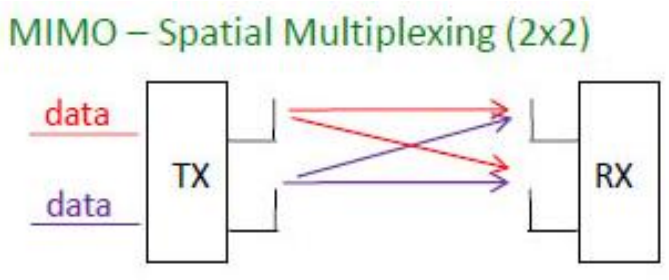
\includegraphics[width=0.4\textwidth]{images/MIMO-01.PNG}
%         \end{center}
%         \item une information va être découpée en plusieurs partie et chaque partie va être envoyée en même temps par plusieurs antennes vers plusieurs récepteurs.
%         \begin{center}
%             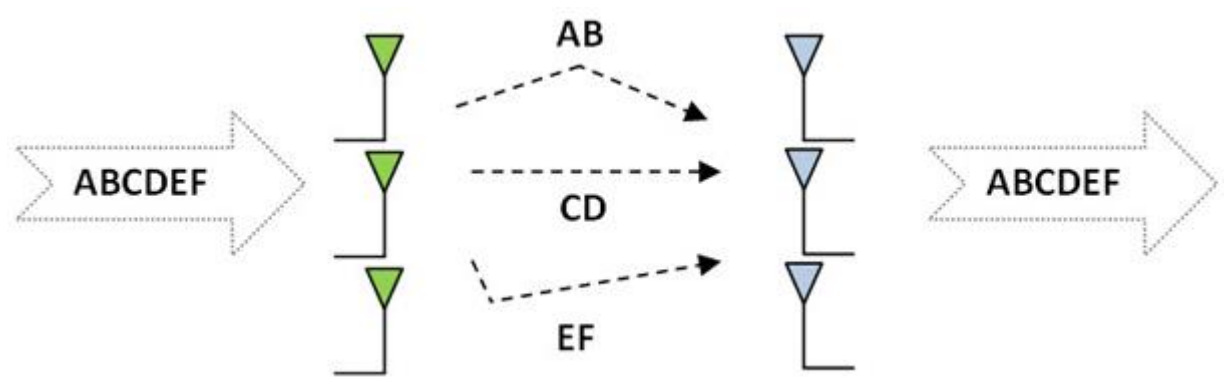
\includegraphics[width=0.6\textwidth]{images/MIMO-2.PNG}
%         \end{center}
%     \end{itemize}
%     \item Amélioration des antennes relais:
%     \begin{itemize}
%         \item antenne relais = station de faible puissance permettant une meilleure couverture du réseau.
%     \end{itemize}
% \end{itemize}





% \subsection{VoLTE}
% \begin{itemize}
%     \item Données et voix sont transportés sous forme de flux IP à condition que le GSM soit compatible VoLTE.
%     \item VoLTE offre une qualité de son HD aux appels et préserve la bande passante radio, ce qui permet d’obtenir un temps de latence moindre par rapport aux services VoIP (Voice over IP) comme Skype.
% \end{itemize}




















%%%%%%%%%%%%%%%%%%%%%%%%%%%%%%%%%%%%%%%%%%%%%%
%%%%                 QCM                  %%%%
%%%%%%%%%%%%%%%%%%%%%%%%%%%%%%%%%%%%%%%%%%%%%%




















\section{QCM}





Les questions sont disponibles sur quizizz \footnote{\texttt{https://quizizz.com/profile/5a92da9a38df4e0021bfee39}}. Il y en aura 20 à l'examen mais il n'y aura pas que des QCM.










\subsection{Les ondes électromagnétiques}





\begin{enumerate}[label=Q\arabic*.]


\item Une onde électromagnétique...
\begin{enumerate}
    \item \textcolor{red}{\textbf{se propage dans le vide.}}
    \item comporte des ondes électrique et magnétique de fréquences différentes.
    \item comporte des ondes électrique et magnétique de périodes différentes.
    \item ne se propage pas dans le vide.
\end{enumerate}


\item Les ondes radios...
\begin{enumerate}
    \item \textcolor{red}{\textbf{ont une longueur d'onde de plus de 1 millimètre.}}
    \item ont une fréquence plus élevée que la celle des rayons X.
    \item ont une longueur d'onde de la taille d'un atome.
    \item ont une fréquence située dans le spectre visible par l’œil humain.
\end{enumerate}


\item Le champ électrique...
\begin{enumerate}
    \item \textcolor{red}{\textbf{varie selon la tension électrique.}}
    \item varie selon le courant électrique.
    \item augmente à mesure que l'on s'éloigne de la source.
    \item se situe tout autour d'un aimant.
\end{enumerate}


\item La longueur d'onde d'une onde électromagnétique...
\begin{enumerate}
    \item \textcolor{red}{\textbf{est la distance parcourue par l'onde pendant une période.}}
    \item se définit en Hertz.
    \item varie tout au long de son parcours.
    \item est d'environ 300 000 km/s.
\end{enumerate}


\item La vitesse de propagation d'une onde électromagnétique dans le vide...
\begin{enumerate}
    \item \textcolor{red}{\textbf{est d'environ 300 000 km/s.}}
    \item dépend de la fréquence de celle-ci.
    \item dépend de la longueur d'onde de celle-ci.
    \item est nulle.
\end{enumerate}


\end{enumerate}










\subsection{Les liaisons hertziennes en espace libre}





\begin{enumerate}[label=Q\arabic*.]


\item  Lorsqu'une onde électromagnétique est réfléchie...
\begin{enumerate}
    \item \textcolor{red}{\textbf{elle est déphasée de 180 degrés.}}
    \item elle est déphasée de 90 degrés.
    \item elle est déphasée de 360 degrés.
    \item elle n'est pas déphasée.
\end{enumerate}


\item Une onde électromagnétique de fréquence comprise entre 3 GHz et 30 GHz...
\begin{enumerate}
    \item \textcolor{red}{\textbf{se propage principalement par onde directe.}}
    \item se propage principalement par onde de sol.
    \item se propage principalement par réflexion dans l'ionosphère (onde de ciel).
    \item ne se propage pas.
\end{enumerate}


\item Lors d'une liaison half-duplex...
\begin{enumerate}
    \item \textcolor{red}{\textbf{l'information circule dans les deux sens mais pas simultanément.}}
    \item l'information ne circule que dans un sens.
    \item l'information circule dans les deux sens simultanément.
    \item il n'y a que la moitié de l'information qui est transmise.
\end{enumerate}


\item Une onde de ciel...
\begin{enumerate}
    \item \textcolor{red}{\textbf{a une portée mondiale mais peut avoir des interférences avec l'onde de sol.}}
    \item a une portée d'environ 500 km.
    \item a besoin que l'émetteur et le récepteur soient en inter-visibilité.
    \item aucune des trois propositions.
\end{enumerate}


\item La propagation d'un signal peu être considéré LOS (en visibilité) si...
\begin{enumerate}
    \item \textcolor{red}{\textbf{60 \% de la zone de Fresnel est libre d'obstacle.}}
    \item 50 \% de la zone de Fresnel est libre d'obstacle.
    \item 40 \% de la zone de Fresnel est libre d'obstacle.
    \item 30 \% d de la zone de Fresnel est libre d'obstacle.
\end{enumerate}


\end{enumerate}










\subsection{Les antennes}





\begin{enumerate}[label=Q\arabic*.]


\item Pour calculer, en décibel, le rapport de 2 puissances, on utilise la formule:
\begin{enumerate}
    \item $\displaystyle \log \frac{P_2}{P_1} $.
    \item \textcolor{red}{\textbf{$\displaystyle 10 \times \log \frac{P_2}{P_1} $}.}
    \item $\displaystyle 20 \times \log \frac{P_2}{P_1} $.
    \item $\displaystyle 30 \times \log \frac{P_2}{P_1} $.
\end{enumerate}


\item Un rapport de puissance de 2 \bigg($\displaystyle \frac{P_2}{P_1} = 2 $\bigg) équivaut à environ...
\begin{enumerate}
    \item 1 dB.
    \item 2 dB.
    \item \textcolor{red}{\textbf{3 dB.}}
    \item 4 dB.
\end{enumerate}


\item La bande passante d'une antenne en réception correspond...
\begin{enumerate}
    \item \textcolor{red}{\textbf{à la plage de fréquences à laquelle l'antenne capte le mieux.}}
    \item au débit de données reçues par l'antenne.
    \item à la taille minimale de l'antenne en fonction de la fréquence de l'onde à recevoir.
    \item à aucune des réponses ci-dessus.
\end{enumerate}


\item  Le gain d'une antenne correspond...
\begin{enumerate}
    \item à la réception d'une antenne après avoir gagné à une tombola.
    \item à l'augmentation du débit de donnée grâce à l'antenne.
    \item \textcolor{red}{\textbf{au fait que le rayonnement est favorisé dans une certaine direction.}}
    \item au gain de puissance d'émission de l'antenne par rapport à la puissance reçue par celle-ci.
\end{enumerate}


\item L'angle d'ouverture d'une antenne...
\begin{enumerate}
    \item est l'angle à l’intérieur duquel la puissance rayonnée ne sera jamais plus faible que la moitié de la puissance maximale rayonnée.
    \item est l'angle à l'intérieur duquel la puissance rayonnée est de -3 dB au minimum par rapport à la puissance maximale.
    \item est l'angle à l'intérieur duquel la puissance rayonnée est la moitié au minimum par rapport à la puissance maximale.
    \item \textcolor{red}{\textbf{est l'angle défini par les trois réponses ci-dessus.}}
\end{enumerate}


\end{enumerate}










\subsection{Signal - Série de Fourier - Spectre}





\begin{enumerate}[label=Q\arabic*.]


\item Dans l'équation: $ x(t) = A \; \cos( \omega t + \varphi) $, $ \omega $ représente:
\begin{enumerate}
    \item \textcolor{red}{\textbf{la pulsation du signal $ x(t) $.}}
    \item l'amplitude du signal $ x(t) $.
    \item la fréquence du signal $ x(t) $.
    \item la phase du signal $ x(t) $.
\end{enumerate}


\item Tout signal périodique...
\begin{enumerate}
    \item ne peut pas être représenté par une série de Fourier.
    \item voit sa fréquence changer en fonction du temps.
    \item \textcolor{red}{\textbf{peut être représenté par une série de Fourier.}}
    \item demande de calculer la transformée de Fourier pour le représenter.
\end{enumerate}


\item Quelle image représente le spectre du signal: $ x(t) = 3 \cos(5 \omega) - 2 \cos(\omega) + 5 \cos(3 \omega) $,
\begin{center} \begin{tabular}{cc}
    (a) & (b) \\
    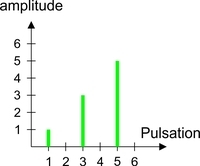
\includegraphics[width=5cm]{images/QCM-4-3-img1.jpg} &
    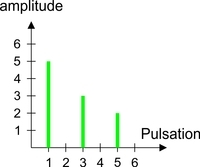
\includegraphics[width=5cm]{images/QCM-4-3-img2.jpg} \\
    (c) & \textcolor{red}{\textbf{(d)}} \\
    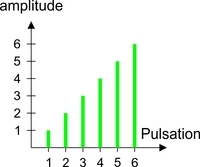
\includegraphics[width=5cm]{images/QCM-4-3-img3.jpg} &
    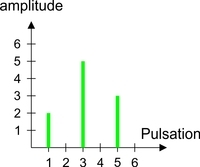
\includegraphics[width=5cm]{images/QCM-4-3-img4.jpg}
\end{tabular} \end{center}


\item La note mi est une onde sinusoïdale qui se répète 330 fois par seconde, on peut donc dire...
\begin{enumerate}
    \item que le mi a une fréquence de 330 Hz, les autres réponses sont fausses.
    \item que le mi a une période de 1/330 seconde, les autres réponses sont fausses.
    \item que le mi est un signal périodique, les autres réponses sont fausses.
    \item \textcolor{red}{\textbf{les 3 réponses ci-dessus sont correctes.}}
\end{enumerate}


\item Un des objectifs recherché en traitant un signal...
\begin{enumerate}
    \item est de réduire le bruit en amplifiant le signal.
    \item est d'étendre le spectre du signal pour améliorer le débit.
    \item \textcolor{red}{\textbf{est de transposer le signal vers les hautes fréquences pour qu'il se propage mieux dans l'air.}}
    \item est de diminuer sa fréquence pour pouvoir utiliser des antennes plus petites.
\end{enumerate}


\end{enumerate}










\subsection{Traitement d'un signal - analogique / numérique}





\begin{enumerate}[label=Q\arabic*.]


\item Dans cette série de Fourier:
\begin{center}
    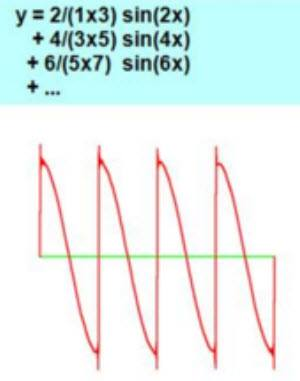
\includegraphics[width=0.35\textwidth]{images/QCM-traitement-signal-01.png}
\end{center}
\begin{enumerate}
    \item l'amplitude du premier terme est 2.
    \item \textcolor{red}{\textbf{l'amplitude du premier terme est 2/3.}}
    \item la fréquence du premier terme est 2 fois plus grande que la fréquence du deuxième terme.
    \item la fréquence du premier terme est 3 fois plus petite que la fréquence du deuxième terme.
\end{enumerate}


\item Un signal est considéré à bande étroite si...
\begin{enumerate}
    \item \textcolor{red}{\textbf{$ \Delta f \ll f_{moy} $ (soit $ f_2 \approx f_1 $)}}
    \item $ \Delta f > f_{moy} $ (soit $ f_2 \gg f_1 $)
\end{enumerate}


\item La transposition de fréquence effectuée à l'aide d'un multiplicateur donnera en sortie un spectre du type:
\begin{center} \begin{tabular}{cc}
    (a) & \textcolor{red}{\textbf{(b)}} \\
    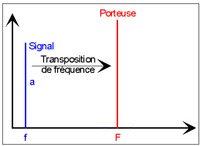
\includegraphics[width=5cm]{images/qcm-5-01.png} &
    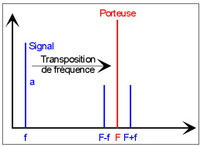
\includegraphics[width=5cm]{images/qcm-5-02.png} \\
    (c) & (d) \\
    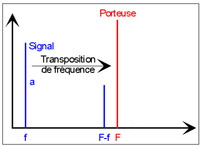
\includegraphics[width=5cm]{images/qcm-5-03.png} &
    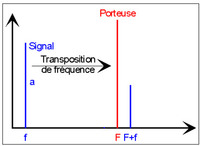
\includegraphics[width=5cm]{images/qcm-5-04.png}
\end{tabular} \end{center}


\item Un signal analogique...
\begin{enumerate}
    \item est un signal à amplitude discrète et temps continu.
    \item est un signal à amplitude et temps discret.
    \item est un signal à amplitude continue et temps discret.
    \item \textcolor{red}{\textbf{est un signal à amplitude et temps continu.}}
\end{enumerate}


\item Le multiplexage fréquentiel...
\begin{enumerate}
    \item permet d'envoyer plusieurs signaux sur la même porteuse.
    \item utilise plusieurs bande de fréquence pour un même signal.
    \item \textcolor{red}{\textbf{sépare les signaux en bandes de fréquences définies dans un plan fréquentiel.}}
    \item sépare les signaux aléatoirement dans des bandes de fréquences différentes.
\end{enumerate}


\end{enumerate}










\subsection{Transmissions numériques et erreurs}





\begin{enumerate}[label=Q\arabic*.]


\item Quel schéma représente la suite de bit 0101 en NRZ-I ?
\begin{center} \begin{tabular}{cc}
    (a) & \textcolor{red}{\textbf{(b)}} \\
    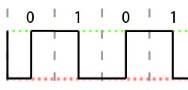
\includegraphics[width=5cm]{images/qcm-6-01.png} &
    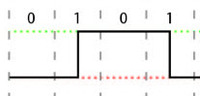
\includegraphics[width=5cm]{images/qcm-6-02.png} \\
    (c) & (d) \\
    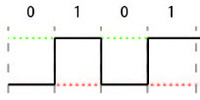
\includegraphics[width=5cm]{images/qcm-6-03.png} &
    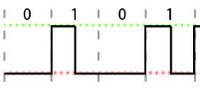
\includegraphics[width=5cm]{images/qcm-6-04.png}
\end{tabular} \end{center}


\item Le code détecteur d'erreur d'un octet en parité impair... (plusieurs réponses possible)
\begin{enumerate}
    \item sera 1 si 1, 3, 5 ou 7 bits sont à 1.
    \item sera 0 si 2, 4, 6 ou 8 bits sont à 1.
    \item \textcolor{red}{\textbf{sera 0 si 1, 3, 5 ou 7 bits sont à 1.}}
    \item \textcolor{red}{\textbf{sera 1 si 2, 4, 6 ou 8 bits sont à 1.}}
\end{enumerate}


\item L'entrelacement permet...
\begin{enumerate}
    \item de minimiser l'impact des erreurs isolées.
    \item d'augmenter le débit de la transmission.
    \item \textcolor{red}{\textbf{de minimiser l'impact d'une salve d'erreurs consécutives.}}
    \item de transposer la fréquence du signal vers les hautes fréquences.
\end{enumerate}


\item La transformation d'information binaire sous forme d'un signal à deux états est réalisée par un...
\begin{enumerate}
    \item modulateur d'amplitude.
    \item oscilloscope.
    \item entrelaceur.
    \item \textcolor{red}{\textbf{codeur bande de base.}}
\end{enumerate}


\item Quel schéma représente la suite de bit 0101 en Manchester ?
\begin{center} \begin{tabular}{cc}
    \textcolor{red}{\textbf{(a)}} & (b) \\
    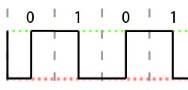
\includegraphics[width=5cm]{images/qcm-6-01.png} &
    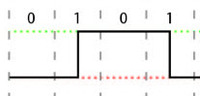
\includegraphics[width=5cm]{images/qcm-6-02.png} \\
    (c) & (d) \\
    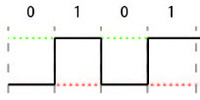
\includegraphics[width=5cm]{images/qcm-6-03.png} &
    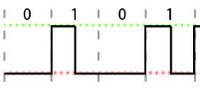
\includegraphics[width=5cm]{images/qcm-6-04.png}
\end{tabular} \end{center}


\end{enumerate}










\subsection{Modulation analogique}





\begin{enumerate}[label=Q\arabic*.]


\item Lors d'une modulation d'amplitude, le signal modulé...
\begin{enumerate}
    \item garde toujours la même amplitude et voit sa fréquence varier.
    \item \textcolor{red}{\textbf{garde toujours la même fréquence et voit son amplitude varier.}}
    \item garde toujours la même amplitude et la même fréquence.
    \item voit son amplitude et sa fréquence varier.
\end{enumerate}


\item On dit, pour un signal AM, qu'il y a surmodulation si...
\begin{enumerate}
    \item \textcolor{red}{\textbf{l'amplitude du message est plus importante que l'amplitude de la porteuse.}}
    \item l'amplitude de la porteuse est plus importante que l'amplitude du signal.
    \item la fréquence du message est plus importante que la fréquence de la porteuse.
    \item la fréquence de la porteuse est plus importante que la fréquence du signal.
\end{enumerate}


\item Lors de la démodulation d'enveloppe d'un signal AM, quel schéma indique une constante de temps du condensateur correcte ?
\begin{center} \begin{tabular}{cc}
    (a) & (b) \\
    \includegraphics[width=5cm]{images/qcm-analogique-001.png} &
    \includegraphics[width=5cm]{images/qcm-analogique-002.png} \\
    \textcolor{red}{\textbf{(c)}} & \\
    \includegraphics[width=5cm]{images/qcm-analogique-003.png} &
\end{tabular} \end{center}


\item L'avantage de la modulation de fréquence par rapport à la modulation d'amplitude... (plusieurs réponses possibles)
\begin{enumerate}
    \item \textcolor{red}{\textbf{est que la puissance du signal modulé reste constante.}}
    \item a une faible largeur de bande.
    \item \textcolor{red}{\textbf{évite le problème de surmodulation.}}
    \item \textcolor{red}{\textbf{permet une moindre sensibilité au bruit.}}
\end{enumerate}


\item L’excursion de fréquence en FM...
\begin{enumerate}
    \item est la variation de fréquence entre la fréquence minimale et maximale du signal modulé.
    \item est la variation de fréquence entre la fréquence minimale et maximale de la porteuse.
    \item est la variation de fréquence entre la fréquence de la porteuse et la fréquence maximale (ou min) du signal modulant.
    \item \textcolor{red}{\textbf{est la variation de fréquence entre la fréquence de la porteuse et la fréquence maximale (ou min) du signal modulé.}}
\end{enumerate}


\end{enumerate}










\subsection{Modulation numérique}





\begin{enumerate}[label=Q\arabic*.]


\item Quelle particularité est vraie lors d'une modulation OOK (On Off Keying) ou ASK (Amplitude Shift Keying) ?
\begin{enumerate}
    \item La puissance émise par la modulation ASK est nulle si le bit est à 1.
    \item La puissance émise par la modulation ASK est nulle si le bit est à 0.
    \item La puissance émise par la modulation OOK est nulle si le bit est à 1.
    \item \textcolor{red}{\textbf{La puissance émise par la modulation OOK est nulle si le bit est à 0.}}
\end{enumerate}


\item Lors d'une modulation AFSK, l'information est transportée à l'aide de différentes fréquences...
\begin{enumerate}
    \item de lumière.
    \item \textcolor{red}{\textbf{de son.}}
    \item de courant.
    \item d'ondes électromagnétiques.
\end{enumerate}


\item Combien de bit(s) par cycle d'horloge sont envoyer à l'aide de la modulation QPSK ?
\begin{enumerate}
    \item 1
    \item \textcolor{red}{\textbf{2}}
    \item 4
    \item 8
\end{enumerate}


\item Combien de bit(s) par cycle d'horloge sont envoyer à l'aide de la modulation 8PSK ?
\begin{enumerate}
    \item 1
    \item 2
    \item \textcolor{red}{\textbf{3}}
    \item 4
\end{enumerate}


\item Quelle affirmation est fausse concernant les modulations 16PSK et 16QAM ?
\begin{enumerate}
    \item Les deux modulations permettent de coder 4 bits par symboles.
    \item Les points de la modulation 16QAM sont plus éloignés → meilleure résistance au bruit.
    \item L'amplitude des points 16QAM les plus éloignés est plus grande → amplificateur plus puissant.
    \item \textcolor{red}{\textbf{Entre deux points de la constellation 16PSK, il y a toujours au moins deux bits qui diffèrent.}}
\end{enumerate}


\end{enumerate}










\subsection{Modulation d'impulsions analogiques}





\begin{enumerate}[label=Q\arabic*.]


\item À quelle fréquence faut-il échantillonner un signal pour garder la qualité de celui-ci ?
\begin{enumerate}
    \item \textcolor{red}{\textbf{au moins 2 fois la fréquence maximale du signal d'information.}}
    \item au moins 2 fois la fréquence minimale du signal d'information.
    \item au moins 6 fois la fréquence maximale du signal d'information.
    \item au moins 6 fois la fréquence minimale du signal d'information.
\end{enumerate}


\item La PWM (modulation par largeur d’impulsion) est une technique de modulation impulsionnelle qui...
\begin{center}
    \includegraphics[width=0.5\textwidth]{images/qcm-9-01.png}
\end{center}
\begin{enumerate}
    \item \textcolor{red}{\textbf{garde l’amplitude constante.}}
    \item \textcolor{red}{\textbf{fait varier la largeur d’impulsion.}}
    \item fait varier la période de l'horloge.
    \item \textcolor{red}{\textbf{garde la fréquence constante.}}
\end{enumerate}


\item La PPM (Pulse Position Modulation) différentielle...
\begin{enumerate}
    \item nécessite d'utiliser une horloge.
    \item génère un signal modulé ayant une amplitude variable.
    \item \textcolor{red}{\textbf{permet la transmission des données indépendamment d'une horloge.}}
    \item est beaucoup moins rapide que le PPM classique.
\end{enumerate}


\item Lors du PCM (Pulse Coded Modulation), l'erreur de quantification est due...
\begin{enumerate}
    \item à la sensibilité des capteurs.
    \item à la fréquence d'horloge.
    \item \textcolor{red}{\textbf{au nombre de bits utilisé lors de la modulation.}}
    \item à la fréquence du signal.
\end{enumerate}


\item Lors de la conversion analogique vers numérique, quelles étapes sont nécessaires ?
\begin{enumerate}
    \item Utiliser des séries de Fourier.
    \item \textcolor{red}{\textbf{Quantifier.}}
    \item \textcolor{red}{\textbf{Supprimer des fréquences.}}
    \item \textcolor{red}{\textbf{Échantillonner.}}
\end{enumerate}


\end{enumerate}










% \subsection{Les courants porteurs en ligne}





% \begin{enumerate}[label=Q\arabic*.]


% \item La technologie des courants porteurs en ligne...
% \begin{enumerate}
%     \item utilise le réseau Ethernet pour faire passer de l’information numérique.
%     \item \textcolor{red}{\textbf{utilise le réseau électrique pour faire passer de l’information numérique.}}
%     \item utilise le réseau optique pour faire passer de l’information numérique.
%     \item utilise le réseau sanitaire pour faire passer de l’information numérique.
% \end{enumerate}


% \item Les adaptateurs CPL, lorsqu'ils reçoivent le signal du réseau électrique...
% \begin{enumerate}
%     \item suppriment les basses tensions.
%     \item suppriment les hautes tensions.
%     \item suppriment les hautes fréquences.
%     \item \textcolor{red}{\textbf{suppriment les basses fréquences.}}
% \end{enumerate}


% \item Lors du multiplexage OFDM (Orthogonal Frequency Division Multiplexing),
% \begin{enumerate}
%     \item \textcolor{red}{\textbf{le signal est réparti sur un grand nombre de sous-porteuses de fréquence distincte.}}
%     \item plusieurs signaux sont réunis sur une sous-porteuses de fréquence bien définie.
%     \item une monoporteuse réalise un multiplexage temporel (chaque signal a un temps pendant lequel la porteuse lui est alloué).
%     \item les signaux sont multiplexés à l'aide de la polarisation de chaque signal.
% \end{enumerate}


% \item Lors de la modulation à étalement de spectre CDMA,
% \begin{enumerate}
%     \item \textcolor{red}{\textbf{chaque liaison utilise son propre code.}}
%     \item \textcolor{red}{\textbf{plusieurs liaisons numériques utilisent simultanément la même fréquence porteuse.}}
%     \item \textcolor{red}{\textbf{si le récepteur ne connaît pas le code des liaisons, il traite le signal comme du bruit.}}
%     \item le signal est réparti sur un grand nombre de sous-porteuses de fréquence distincte.
% \end{enumerate}


% \item Le CPL outdoor...
% \begin{enumerate}
%     \item nécessite une coopération entre le distributeur d'eau et le fournisseur d'accès internet.
%     \item \textcolor{red}{\textbf{nécessite une coopération entre le distributeur d'électricité et le fournisseur d'accès internet.}}
%     \item nécessite une coopération entre le distributeur d'électricité et le fournisseur d'eau.
%     \item nécessite une coopération entre le distributeur d'électricité et le fournisseur de gaz.
% \end{enumerate}


% \end{enumerate}










\subsection{La fibre optique}





\begin{enumerate}[label=Q\arabic*.]


\item Au regard du graphique, quelle sera la longueur d'onde a choisir pour minimiser l'atténuation de la lumière dans la fibre optique ?
\begin{center}
    \includegraphics[width=0.55\textwidth]{images/fibre-6.PNG}
\end{center}
\begin{enumerate}
    \item \textcolor{red}{\textbf{1550 nm.}}
    \item 1.4 $ \mu $m.
    \item 900 nm.
    \item 15 THz.
\end{enumerate}


\item Lorsqu'une impulsion lumineuse composée de plusieurs longueur d'onde transite dans une fibre optique...
\begin{enumerate}
    \item seule une longueur d'onde atteint le bout de la fibre.
    \item \textcolor{red}{\textbf{cela veut dire que la source de l’impulsion est une LED.}}
    \item toutes les longueurs d'onde de l’impulsion arrivent exactement au même moment au bout de la fibre.
    \item \textcolor{red}{\textbf{certaines longueurs d'ondes arrivent avant d'autres et l’impulsion s’étale dans le temps.}}
\end{enumerate}


\item Lors du multiplexage WDM (Wavelength Division multiplexing)...
\begin{enumerate}
    \item chaque signal utilise la totalité de la bande passante pendant un court instant et ce à tour de rôle pour chaque signal.
    \item les amplitudes des signaux à multiplexer sont additionnées pour former un seul signal.
    \item les fréquences des signaux à multiplexer sont additionnées pour former un seul signal.
    \item \textcolor{red}{\textbf{les signaux sont portés par des longueurs d'ondes différentes, et espacées assez largement afin de ne pas interférer les unes avec les autres.}}
\end{enumerate}


\item La fibre optique mono-mode...
\begin{enumerate}
    \item \textcolor{red}{\textbf{a la particularité d'avoir un cœur avec un diamètre beaucoup plus petit qu'une fibre multi-mode.}}
    \item \textcolor{red}{\textbf{permet théoriquement au signal lumineux de se déplacer en ligne droite.}}
    \item a comme particularité d'avoir l'indice de réfraction qui varie dans l'épaisseur du cœur de manière graduelle.
    \item n’accepte que les fréquences en dessous du kHz.
\end{enumerate}


\item La particularité d'un émetteur LED par rapport à un émetteur laser est...
\begin{enumerate}
    \item qu'il ne s'utilise que pour les fibres monomode.
    \item qu'il permet des débit de transmission beaucoup plus élevé.
    \item \textcolor{red}{\textbf{que sa puissance de consommation est plus faible.}}
    \item qu'il est beaucoup plus cher.
\end{enumerate}


\end{enumerate}










% \subsection{La 4G et 4G+}





% \begin{enumerate}[label=Q\arabic*.]


% \item Les largeurs de bandes disponibles dans la technologie 4G sont généralement au nombre de...
% \begin{enumerate}
%     \item 2
%     \item \textcolor{red}{\textbf{6}}
%     \item 25
%     \item 150
% \end{enumerate}


% \item En 4G, une bande de fréquence ayant une largeur de 20 MHz possède 100 ressources blocks. Il peut donc transmettre 100*84 symboles * 6 bits transmis en 0,5 ms. Quel en sera le débit en bits/s ?
% \begin{enumerate}
%     \item 100,8 Kbits/s.
%     \item 1008 Mbits/s.
%     \item 10,8 Mbits/s.
%     \item \textcolor{red}{\textbf{100,8 Mbits/s.}}
% \end{enumerate}


% \item Les nouvelles fonctionnalités de la 4G+ par rapport à la 4G sont, entre autre:
% \begin{enumerate}
%     \item \textcolor{red}{\textbf{L'utilisation de plusieurs bande de fréquence pour une seule transmission.}}
%     \item \textcolor{red}{\textbf{Une meilleure utilisation de la technique "Multiple Input Multiple Output" (MIMO).}}
%     \item La puissance émise par les antennes est beaucoup plus élevée.
%     \item La hauteur des antennes relais est beaucoup plus élevée.
% \end{enumerate}


% \item Lors de la technologie MIMO (Multiple Input Multiple Output)...
% \begin{enumerate}
%     \item l'information partira d'un émetteur vers un récepteur.
%     \item l'information partira de plusieurs émetteurs vers un récepteur.
%     \item \textcolor{red}{\textbf{l'information partira de plusieurs émetteurs vers plusieurs récepteurs.}}
%     \item l'information partira d'un émetteur vers plusieurs récepteurs.
% \end{enumerate}


% \item Que veut dire l’acronyme VoLTE ?
% \begin{enumerate}
%     \item Vibration over LTE.
%     \item \textcolor{red}{\textbf{Voice over LTE.}}
%     \item Validation over LTE.
%     \item Vercingetorix over LTE.
% \end{enumerate}


% \end{enumerate}



















\newpage \tableofcontents

\end{document}